\documentclass[a4paper]{article}
\usepackage{geometry}
\usepackage{booktabs}
\usepackage{tikz}
\usepackage{ytableau}
\usepackage{hyperref}
\usepackage{fancyhdr}
\usepackage{multicol}
\geometry{margin=0.5in}
\pagestyle{fancy}
\fancyhf{}
\fancyhead[L]{Header}
\fancyfoot[C]{\thepage}
\begin{document}
\tableofcontents
\newpage
\section{Genus 1}
\newpage\subsection{MinGens: [2, 3]}
\subsubsection*{Invariants}
\begin{minipage}{0.48\textwidth}
\begin{tabular}{|c|c|c|c|c|c|c|}
\toprule
g & F & m & ewt & t & \(|M|\) & \(|\lambda|\) \\
\midrule
1 & 1 & 2 & 0 & 1 & 0 & 1 \\
\bottomrule
\end{tabular}
\end{minipage}
\subsubsection*{Partition}
\begin{minipage}{0.48\textwidth}
\begin{tikzpicture}
  \draw (0.00, 0.00) rectangle (0.20, -0.20);
\end{tikzpicture}
\end{minipage}
\subsubsection*{Gap Poset}
\begin{minipage}{0.48\textwidth}
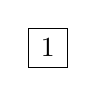
\begin{tikzpicture}
  \node[draw, rectangle, minimum size=0.5cm] (1) at (0.00,0.00) {1};
\end{tikzpicture}
\end{minipage}
\subsubsection*{Void Poset}
\begin{minipage}{0.48\textwidth}
\end{minipage}
\section{Genus 2}
\newpage\subsection{MinGens: [3, 4, 5]}
\subsubsection*{Invariants}
\begin{minipage}{0.48\textwidth}
\begin{tabular}{|c|c|c|c|c|c|c|}
\toprule
g & F & m & ewt & t & \(|M|\) & \(|\lambda|\) \\
\midrule
2 & 2 & 3 & 0 & 2 & 1 & 2 \\
\bottomrule
\end{tabular}
\end{minipage}
\subsubsection*{Partition}
\begin{minipage}{0.48\textwidth}
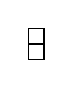
\begin{tikzpicture}
  \draw (0.00, 0.00) rectangle (0.20, -0.20);
  \draw (0.00, -0.20) rectangle (0.20, -0.40);
\end{tikzpicture}
\end{minipage}
\subsubsection*{Gap Poset}
\begin{minipage}{0.48\textwidth}
\begin{tikzpicture}
  \node[minimum size=0.5cm] (1) at (0.00,0.00) {1};
  \node[draw, rectangle, minimum size=0.5cm] (2) at (2.00,0.00) {2};
\end{tikzpicture}
\end{minipage}
\subsubsection*{Void Poset}
\begin{minipage}{0.48\textwidth}
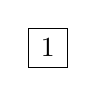
\begin{tikzpicture}
  \node[draw, rectangle, minimum size=0.5cm] (1) at (0.00,0.00) {1};
\end{tikzpicture}
\end{minipage}
\newpage\subsection{MinGens: [2, 5]}
\subsubsection*{Invariants}
\begin{minipage}{0.48\textwidth}
\begin{tabular}{|c|c|c|c|c|c|c|}
\toprule
g & F & m & ewt & t & \(|M|\) & \(|\lambda|\) \\
\midrule
2 & 3 & 2 & 1 & 1 & 0 & 3 \\
\bottomrule
\end{tabular}
\end{minipage}
\subsubsection*{Partition}
\begin{minipage}{0.48\textwidth}
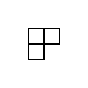
\begin{tikzpicture}
  \draw (0.00, 0.00) rectangle (0.20, -0.20);
  \draw (0.20, 0.00) rectangle (0.40, -0.20);
  \draw (0.00, -0.20) rectangle (0.20, -0.40);
\end{tikzpicture}
\end{minipage}
\subsubsection*{Gap Poset}
\begin{minipage}{0.48\textwidth}
\begin{tikzpicture}
  \node[minimum size=0.5cm] (1) at (0.00,-2.00) {1};
  \node[draw, rectangle, minimum size=0.5cm] (3) at (0.00,0.00) {3};
  % Draw the cover relations
  \draw (3) -- (1);
\end{tikzpicture}
\end{minipage}
\subsubsection*{Void Poset}
\begin{minipage}{0.48\textwidth}
\end{minipage}
\section{Genus 3}
\newpage\subsection{MinGens: [4, 5, 6, 7]}
\subsubsection*{Invariants}
\begin{minipage}{0.48\textwidth}
\begin{tabular}{|c|c|c|c|c|c|c|}
\toprule
g & F & m & ewt & t & \(|M|\) & \(|\lambda|\) \\
\midrule
3 & 3 & 4 & 0 & 3 & 2 & 3 \\
\bottomrule
\end{tabular}
\end{minipage}
\subsubsection*{Partition}
\begin{minipage}{0.48\textwidth}
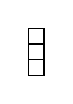
\begin{tikzpicture}
  \draw (0.00, 0.00) rectangle (0.20, -0.20);
  \draw (0.00, -0.20) rectangle (0.20, -0.40);
  \draw (0.00, -0.40) rectangle (0.20, -0.60);
\end{tikzpicture}
\end{minipage}
\subsubsection*{Gap Poset}
\begin{minipage}{0.48\textwidth}
\begin{tikzpicture}
  \node[minimum size=0.5cm] (1) at (0.00,0.00) {1};
  \node[minimum size=0.5cm] (2) at (2.00,0.00) {2};
  \node[draw, rectangle, minimum size=0.5cm] (3) at (4.00,0.00) {3};
\end{tikzpicture}
\end{minipage}
\subsubsection*{Void Poset}
\begin{minipage}{0.48\textwidth}
\begin{tikzpicture}
  \node[minimum size=0.5cm] (1) at (0.00,0.00) {1};
  \node[draw, rectangle, minimum size=0.5cm] (2) at (2.00,0.00) {2};
\end{tikzpicture}
\end{minipage}
\newpage\subsection{MinGens: [3, 5, 7]}
\subsubsection*{Invariants}
\begin{minipage}{0.48\textwidth}
\begin{tabular}{|c|c|c|c|c|c|c|}
\toprule
g & F & m & ewt & t & \(|M|\) & \(|\lambda|\) \\
\midrule
3 & 4 & 3 & 1 & 2 & 1 & 4 \\
\bottomrule
\end{tabular}
\end{minipage}
\subsubsection*{Partition}
\begin{minipage}{0.48\textwidth}
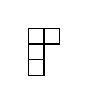
\begin{tikzpicture}
  \draw (0.00, 0.00) rectangle (0.20, -0.20);
  \draw (0.20, 0.00) rectangle (0.40, -0.20);
  \draw (0.00, -0.20) rectangle (0.20, -0.40);
  \draw (0.00, -0.40) rectangle (0.20, -0.60);
\end{tikzpicture}
\end{minipage}
\subsubsection*{Gap Poset}
\begin{minipage}{0.48\textwidth}
\begin{tikzpicture}
  \node[minimum size=0.5cm] (1) at (0.00,-2.00) {1};
  \node[minimum size=0.5cm] (2) at (0.00,0.00) {2};
  \node[draw, rectangle, minimum size=0.5cm] (4) at (2.00,0.00) {4};
  % Draw the cover relations
  \draw (4) -- (1);
\end{tikzpicture}
\end{minipage}
\subsubsection*{Void Poset}
\begin{minipage}{0.48\textwidth}
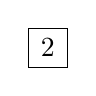
\begin{tikzpicture}
  \node[draw, rectangle, minimum size=0.5cm] (2) at (0.00,0.00) {2};
\end{tikzpicture}
\end{minipage}
\newpage\subsection{MinGens: [3, 4]}
\subsubsection*{Invariants}
\begin{minipage}{0.48\textwidth}
\begin{tabular}{|c|c|c|c|c|c|c|}
\toprule
g & F & m & ewt & t & \(|M|\) & \(|\lambda|\) \\
\midrule
3 & 5 & 3 & 2 & 1 & 0 & 5 \\
\bottomrule
\end{tabular}
\end{minipage}
\subsubsection*{Partition}
\begin{minipage}{0.48\textwidth}
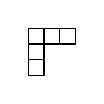
\begin{tikzpicture}
  \draw (0.00, 0.00) rectangle (0.20, -0.20);
  \draw (0.20, 0.00) rectangle (0.40, -0.20);
  \draw (0.40, 0.00) rectangle (0.60, -0.20);
  \draw (0.00, -0.20) rectangle (0.20, -0.40);
  \draw (0.00, -0.40) rectangle (0.20, -0.60);
\end{tikzpicture}
\end{minipage}
\subsubsection*{Gap Poset}
\begin{minipage}{0.48\textwidth}
\begin{tikzpicture}
  \node[minimum size=0.5cm] (1) at (0.00,-2.00) {1};
  \node[minimum size=0.5cm] (2) at (2.00,-2.00) {2};
  \node[draw, rectangle, minimum size=0.5cm] (5) at (0.00,0.00) {5};
  % Draw the cover relations
  \draw (5) -- (1);
  \draw (5) -- (2);
\end{tikzpicture}
\end{minipage}
\subsubsection*{Void Poset}
\begin{minipage}{0.48\textwidth}
\end{minipage}
\newpage\subsection{MinGens: [2, 7]}
\subsubsection*{Invariants}
\begin{minipage}{0.48\textwidth}
\begin{tabular}{|c|c|c|c|c|c|c|}
\toprule
g & F & m & ewt & t & \(|M|\) & \(|\lambda|\) \\
\midrule
3 & 5 & 2 & 2 & 1 & 0 & 6 \\
\bottomrule
\end{tabular}
\end{minipage}
\subsubsection*{Partition}
\begin{minipage}{0.48\textwidth}
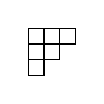
\begin{tikzpicture}
  \draw (0.00, 0.00) rectangle (0.20, -0.20);
  \draw (0.20, 0.00) rectangle (0.40, -0.20);
  \draw (0.40, 0.00) rectangle (0.60, -0.20);
  \draw (0.00, -0.20) rectangle (0.20, -0.40);
  \draw (0.20, -0.20) rectangle (0.40, -0.40);
  \draw (0.00, -0.40) rectangle (0.20, -0.60);
\end{tikzpicture}
\end{minipage}
\subsubsection*{Gap Poset}
\begin{minipage}{0.48\textwidth}
\begin{tikzpicture}
  \node[minimum size=0.5cm] (1) at (0.00,-4.00) {1};
  \node[minimum size=0.5cm] (3) at (0.00,-2.00) {3};
  \node[draw, rectangle, minimum size=0.5cm] (5) at (0.00,0.00) {5};
  % Draw the cover relations
  \draw (3) -- (1);
  \draw (5) -- (3);
\end{tikzpicture}
\end{minipage}
\subsubsection*{Void Poset}
\begin{minipage}{0.48\textwidth}
\end{minipage}
\section{Genus 4}
\newpage\subsection{MinGens: [5, 6, 7, 8, 9]}
\subsubsection*{Invariants}
\begin{minipage}{0.48\textwidth}
\begin{tabular}{|c|c|c|c|c|c|c|}
\toprule
g & F & m & ewt & t & \(|M|\) & \(|\lambda|\) \\
\midrule
4 & 4 & 5 & 0 & 4 & 3 & 4 \\
\bottomrule
\end{tabular}
\end{minipage}
\subsubsection*{Partition}
\begin{minipage}{0.48\textwidth}
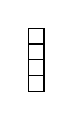
\begin{tikzpicture}
  \draw (0.00, 0.00) rectangle (0.20, -0.20);
  \draw (0.00, -0.20) rectangle (0.20, -0.40);
  \draw (0.00, -0.40) rectangle (0.20, -0.60);
  \draw (0.00, -0.60) rectangle (0.20, -0.80);
\end{tikzpicture}
\end{minipage}
\subsubsection*{Gap Poset}
\begin{minipage}{0.48\textwidth}
\begin{tikzpicture}
  \node[minimum size=0.5cm] (1) at (0.00,0.00) {1};
  \node[minimum size=0.5cm] (2) at (2.00,0.00) {2};
  \node[minimum size=0.5cm] (3) at (4.00,0.00) {3};
  \node[draw, rectangle, minimum size=0.5cm] (4) at (6.00,0.00) {4};
\end{tikzpicture}
\end{minipage}
\subsubsection*{Void Poset}
\begin{minipage}{0.48\textwidth}
\begin{tikzpicture}
  \node[minimum size=0.5cm] (1) at (0.00,0.00) {1};
  \node[minimum size=0.5cm] (2) at (2.00,0.00) {2};
  \node[draw, rectangle, minimum size=0.5cm] (3) at (4.00,0.00) {3};
\end{tikzpicture}
\end{minipage}
\newpage\subsection{MinGens: [4, 6, 7, 9]}
\subsubsection*{Invariants}
\begin{minipage}{0.48\textwidth}
\begin{tabular}{|c|c|c|c|c|c|c|}
\toprule
g & F & m & ewt & t & \(|M|\) & \(|\lambda|\) \\
\midrule
4 & 5 & 4 & 1 & 3 & 2 & 5 \\
\bottomrule
\end{tabular}
\end{minipage}
\subsubsection*{Partition}
\begin{minipage}{0.48\textwidth}
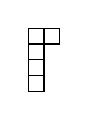
\begin{tikzpicture}
  \draw (0.00, 0.00) rectangle (0.20, -0.20);
  \draw (0.20, 0.00) rectangle (0.40, -0.20);
  \draw (0.00, -0.20) rectangle (0.20, -0.40);
  \draw (0.00, -0.40) rectangle (0.20, -0.60);
  \draw (0.00, -0.60) rectangle (0.20, -0.80);
\end{tikzpicture}
\end{minipage}
\subsubsection*{Gap Poset}
\begin{minipage}{0.48\textwidth}
\begin{tikzpicture}
  \node[minimum size=0.5cm] (1) at (0.00,-2.00) {1};
  \node[minimum size=0.5cm] (2) at (0.00,0.00) {2};
  \node[minimum size=0.5cm] (3) at (2.00,0.00) {3};
  \node[draw, rectangle, minimum size=0.5cm] (5) at (4.00,0.00) {5};
  % Draw the cover relations
  \draw (5) -- (1);
\end{tikzpicture}
\end{minipage}
\subsubsection*{Void Poset}
\begin{minipage}{0.48\textwidth}
\begin{tikzpicture}
  \node[minimum size=0.5cm] (2) at (0.00,0.00) {2};
  \node[draw, rectangle, minimum size=0.5cm] (3) at (2.00,0.00) {3};
\end{tikzpicture}
\end{minipage}
\newpage\subsection{MinGens: [4, 5, 7]}
\subsubsection*{Invariants}
\begin{minipage}{0.48\textwidth}
\begin{tabular}{|c|c|c|c|c|c|c|}
\toprule
g & F & m & ewt & t & \(|M|\) & \(|\lambda|\) \\
\midrule
4 & 6 & 4 & 2 & 2 & 1 & 6 \\
\bottomrule
\end{tabular}
\end{minipage}
\subsubsection*{Partition}
\begin{minipage}{0.48\textwidth}
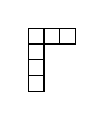
\begin{tikzpicture}
  \draw (0.00, 0.00) rectangle (0.20, -0.20);
  \draw (0.20, 0.00) rectangle (0.40, -0.20);
  \draw (0.40, 0.00) rectangle (0.60, -0.20);
  \draw (0.00, -0.20) rectangle (0.20, -0.40);
  \draw (0.00, -0.40) rectangle (0.20, -0.60);
  \draw (0.00, -0.60) rectangle (0.20, -0.80);
\end{tikzpicture}
\end{minipage}
\subsubsection*{Gap Poset}
\begin{minipage}{0.48\textwidth}
\begin{tikzpicture}
  \node[minimum size=0.5cm] (1) at (0.00,-2.00) {1};
  \node[minimum size=0.5cm] (2) at (2.00,-2.00) {2};
  \node[minimum size=0.5cm] (3) at (0.00,0.00) {3};
  \node[draw, rectangle, minimum size=0.5cm] (6) at (2.00,0.00) {6};
  % Draw the cover relations
  \draw (6) -- (1);
  \draw (6) -- (2);
\end{tikzpicture}
\end{minipage}
\subsubsection*{Void Poset}
\begin{minipage}{0.48\textwidth}

\begin{tikzpicture}
  \node[draw, rectangle, minimum size=0.5cm] (3) at (0.00,0.00) {3};
\end{tikzpicture}
\end{minipage}
\newpage\subsection{MinGens: [4, 5, 6]}
\subsubsection*{Invariants}
\begin{minipage}{0.48\textwidth}
\begin{tabular}{|c|c|c|c|c|c|c|}
\toprule
g & F & m & ewt & t & \(|M|\) & \(|\lambda|\) \\
\midrule
4 & 7 & 4 & 3 & 1 & 0 & 7 \\
\bottomrule
\end{tabular}
\end{minipage}
\subsubsection*{Partition}
\begin{minipage}{0.48\textwidth}
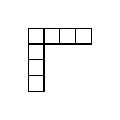
\begin{tikzpicture}
  \draw (0.00, 0.00) rectangle (0.20, -0.20);
  \draw (0.20, 0.00) rectangle (0.40, -0.20);
  \draw (0.40, 0.00) rectangle (0.60, -0.20);
  \draw (0.60, 0.00) rectangle (0.80, -0.20);
  \draw (0.00, -0.20) rectangle (0.20, -0.40);
  \draw (0.00, -0.40) rectangle (0.20, -0.60);
  \draw (0.00, -0.60) rectangle (0.20, -0.80);
\end{tikzpicture}
\end{minipage}
\subsubsection*{Gap Poset}
\begin{minipage}{0.48\textwidth}
\begin{tikzpicture}
  \node[minimum size=0.5cm] (1) at (0.00,-2.00) {1};
  \node[minimum size=0.5cm] (2) at (2.00,-2.00) {2};
  \node[minimum size=0.5cm] (3) at (4.00,-2.00) {3};
  \node[draw, rectangle, minimum size=0.5cm] (7) at (0.00,0.00) {7};
  % Draw the cover relations
  \draw (7) -- (1);
  \draw (7) -- (2);
  \draw (7) -- (3);
\end{tikzpicture}
\end{minipage}
\subsubsection*{Void Poset}
\begin{minipage}{0.48\textwidth}
\end{minipage}
\newpage\subsection{MinGens: [3, 7, 8]}
\subsubsection*{Invariants}
\begin{minipage}{0.48\textwidth}
\begin{tabular}{|c|c|c|c|c|c|c|}
\toprule
g & F & m & ewt & t & \(|M|\) & \(|\lambda|\) \\
\midrule
4 & 5 & 3 & 2 & 2 & 2 & 6 \\
\bottomrule
\end{tabular}
\end{minipage}
\subsubsection*{Partition}
\begin{minipage}{0.48\textwidth}
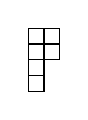
\begin{tikzpicture}
  \draw (0.00, 0.00) rectangle (0.20, -0.20);
  \draw (0.20, 0.00) rectangle (0.40, -0.20);
  \draw (0.00, -0.20) rectangle (0.20, -0.40);
  \draw (0.20, -0.20) rectangle (0.40, -0.40);
  \draw (0.00, -0.40) rectangle (0.20, -0.60);
  \draw (0.00, -0.60) rectangle (0.20, -0.80);
\end{tikzpicture}
\end{minipage}
\subsubsection*{Gap Poset}
\begin{minipage}{0.48\textwidth}
\begin{tikzpicture}
  \node[minimum size=0.5cm] (1) at (0.00,-2.00) {1};
  \node[minimum size=0.5cm] (2) at (2.00,-2.00) {2};
  \node[minimum size=0.5cm] (4) at (0.00,0.00) {4};
  \node[draw, rectangle, minimum size=0.5cm] (5) at (2.00,0.00) {5};
  % Draw the cover relations
  \draw (4) -- (1);
  \draw (5) -- (2);
\end{tikzpicture}
\end{minipage}
\subsubsection*{Void Poset}
\begin{minipage}{0.48\textwidth}
\begin{tikzpicture}
  \node[minimum size=0.5cm] (1) at (0.00,-2.00) {1};
  \node[draw, rectangle, minimum size=0.5cm] (4) at (0.00,0.00) {4};
  % Draw the cover relations
  \draw (4) -- (1);
\end{tikzpicture}
\end{minipage}
\newpage\subsection{MinGens: [3, 5]}
\subsubsection*{Invariants}
\begin{minipage}{0.48\textwidth}
\begin{tabular}{|c|c|c|c|c|c|c|}
\toprule
g & F & m & ewt & t & \(|M|\) & \(|\lambda|\) \\
\midrule
4 & 7 & 3 & 3 & 1 & 0 & 8 \\
\bottomrule
\end{tabular}
\end{minipage}
\subsubsection*{Partition}
\begin{minipage}{0.48\textwidth}
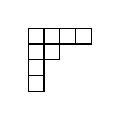
\begin{tikzpicture}
  \draw (0.00, 0.00) rectangle (0.20, -0.20);
  \draw (0.20, 0.00) rectangle (0.40, -0.20);
  \draw (0.40, 0.00) rectangle (0.60, -0.20);
  \draw (0.60, 0.00) rectangle (0.80, -0.20);
  \draw (0.00, -0.20) rectangle (0.20, -0.40);
  \draw (0.20, -0.20) rectangle (0.40, -0.40);
  \draw (0.00, -0.40) rectangle (0.20, -0.60);
  \draw (0.00, -0.60) rectangle (0.20, -0.80);
\end{tikzpicture}
\end{minipage}
\subsubsection*{Gap Poset}
\begin{minipage}{0.48\textwidth}
\begin{tikzpicture}
  \node[minimum size=0.5cm] (1) at (0.00,-4.00) {1};
  \node[minimum size=0.5cm] (2) at (0.00,-2.00) {2};
  \node[minimum size=0.5cm] (4) at (2.00,-2.00) {4};
  \node[draw, rectangle, minimum size=0.5cm] (7) at (0.00,0.00) {7};
  % Draw the cover relations
  \draw (7) -- (4);
  \draw (4) -- (1);
  \draw (7) -- (2);
\end{tikzpicture}
\end{minipage}
\subsubsection*{Void Poset}
\begin{minipage}{0.48\textwidth}
\end{minipage}
\newpage\subsection{MinGens: [2, 9]}
\subsubsection*{Invariants}
\begin{minipage}{0.48\textwidth}
\begin{tabular}{|c|c|c|c|c|c|c|}
\toprule
g & F & m & ewt & t & \(|M|\) & \(|\lambda|\) \\
\midrule
4 & 7 & 2 & 3 & 1 & 0 & 10 \\
\bottomrule
\end{tabular}
\end{minipage}
\subsubsection*{Partition}
\begin{minipage}{0.48\textwidth}
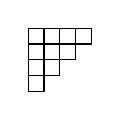
\begin{tikzpicture}
  \draw (0.00, 0.00) rectangle (0.20, -0.20);
  \draw (0.20, 0.00) rectangle (0.40, -0.20);
  \draw (0.40, 0.00) rectangle (0.60, -0.20);
  \draw (0.60, 0.00) rectangle (0.80, -0.20);
  \draw (0.00, -0.20) rectangle (0.20, -0.40);
  \draw (0.20, -0.20) rectangle (0.40, -0.40);
  \draw (0.40, -0.20) rectangle (0.60, -0.40);
  \draw (0.00, -0.40) rectangle (0.20, -0.60);
  \draw (0.20, -0.40) rectangle (0.40, -0.60);
  \draw (0.00, -0.60) rectangle (0.20, -0.80);
\end{tikzpicture}
\end{minipage}
\subsubsection*{Gap Poset}
\begin{minipage}{0.48\textwidth}
\begin{tikzpicture}
  \node[minimum size=0.5cm] (1) at (0.00,-6.00) {1};
  \node[minimum size=0.5cm] (3) at (0.00,-4.00) {3};
  \node[minimum size=0.5cm] (5) at (0.00,-2.00) {5};
  \node[draw, rectangle, minimum size=0.5cm] (7) at (0.00,0.00) {7};
  % Draw the cover relations
  \draw (3) -- (1);
  \draw (5) -- (3);
  \draw (7) -- (5);
\end{tikzpicture}
\end{minipage}
\subsubsection*{Void Poset}
\begin{minipage}{0.48\textwidth}
\end{minipage}
\section{Genus 5}
\newpage\subsection{MinGens: [6, 7, 8, 9, 10, 11]}
\subsubsection*{Invariants}
\begin{minipage}{0.48\textwidth}
\begin{tabular}{|c|c|c|c|c|c|c|}
\toprule
g & F & m & ewt & t & \(|M|\) & \(|\lambda|\) \\
\midrule
5 & 5 & 6 & 0 & 5 & 4 & 5 \\
\bottomrule
\end{tabular}
\end{minipage}
\subsubsection*{Partition}
\begin{minipage}{0.48\textwidth}
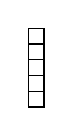
\begin{tikzpicture}
  \draw (0.00, 0.00) rectangle (0.20, -0.20);
  \draw (0.00, -0.20) rectangle (0.20, -0.40);
  \draw (0.00, -0.40) rectangle (0.20, -0.60);
  \draw (0.00, -0.60) rectangle (0.20, -0.80);
  \draw (0.00, -0.80) rectangle (0.20, -1.00);
\end{tikzpicture}
\end{minipage}
\subsubsection*{Gap Poset}
\begin{minipage}{0.48\textwidth}
\begin{tikzpicture}
  \node[minimum size=0.5cm] (1) at (0.00,0.00) {1};
  \node[minimum size=0.5cm] (2) at (2.00,0.00) {2};
  \node[minimum size=0.5cm] (3) at (4.00,0.00) {3};
  \node[minimum size=0.5cm] (4) at (6.00,0.00) {4};
  \node[draw, rectangle, minimum size=0.5cm] (5) at (8.00,0.00) {5};
\end{tikzpicture}
\end{minipage}
\subsubsection*{Void Poset}
\begin{minipage}{0.48\textwidth}
\begin{tikzpicture}
  \node[minimum size=0.5cm] (1) at (0.00,0.00) {1};
  \node[minimum size=0.5cm] (2) at (2.00,0.00) {2};
  \node[minimum size=0.5cm] (3) at (4.00,0.00) {3};
  \node[draw, rectangle, minimum size=0.5cm] (4) at (6.00,0.00) {4};
\end{tikzpicture}
\end{minipage}
\newpage\subsection{MinGens: [5, 7, 8, 9, 11]}
\subsubsection*{Invariants}
\begin{minipage}{0.48\textwidth}
\begin{tabular}{|c|c|c|c|c|c|c|}
\toprule
g & F & m & ewt & t & \(|M|\) & \(|\lambda|\) \\
\midrule
5 & 6 & 5 & 1 & 4 & 3 & 6 \\
\bottomrule
\end{tabular}
\end{minipage}
\subsubsection*{Partition}
\begin{minipage}{0.48\textwidth}
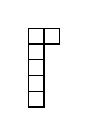
\begin{tikzpicture}
  \draw (0.00, 0.00) rectangle (0.20, -0.20);
  \draw (0.20, 0.00) rectangle (0.40, -0.20);
  \draw (0.00, -0.20) rectangle (0.20, -0.40);
  \draw (0.00, -0.40) rectangle (0.20, -0.60);
  \draw (0.00, -0.60) rectangle (0.20, -0.80);
  \draw (0.00, -0.80) rectangle (0.20, -1.00);
\end{tikzpicture}
\end{minipage}
\subsubsection*{Gap Poset}
\begin{minipage}{0.48\textwidth}
\begin{tikzpicture}
  \node[minimum size=0.5cm] (1) at (0.00,-2.00) {1};
  \node[minimum size=0.5cm] (2) at (0.00,0.00) {2};
  \node[minimum size=0.5cm] (3) at (2.00,0.00) {3};
  \node[minimum size=0.5cm] (4) at (4.00,0.00) {4};
  \node[draw, rectangle, minimum size=0.5cm] (6) at (6.00,0.00) {6};
  % Draw the cover relations
  \draw (6) -- (1);
\end{tikzpicture}
\end{minipage}
\subsubsection*{Void Poset}
\begin{minipage}{0.48\textwidth}
\begin{tikzpicture}
  \node[minimum size=0.5cm] (2) at (0.00,0.00) {2};
  \node[minimum size=0.5cm] (3) at (2.00,0.00) {3};
  \node[draw, rectangle, minimum size=0.5cm] (4) at (4.00,0.00) {4};
\end{tikzpicture}
\end{minipage}
\newpage\subsection{MinGens: [5, 6, 8, 9]}
\subsubsection*{Invariants}
\begin{minipage}{0.48\textwidth}
\begin{tabular}{|c|c|c|c|c|c|c|}
\toprule
g & F & m & ewt & t & \(|M|\) & \(|\lambda|\) \\
\midrule
5 & 7 & 5 & 2 & 3 & 2 & 7 \\
\bottomrule
\end{tabular}
\end{minipage}
\subsubsection*{Partition}
\begin{minipage}{0.48\textwidth}
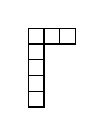
\begin{tikzpicture}
  \draw (0.00, 0.00) rectangle (0.20, -0.20);
  \draw (0.20, 0.00) rectangle (0.40, -0.20);
  \draw (0.40, 0.00) rectangle (0.60, -0.20);
  \draw (0.00, -0.20) rectangle (0.20, -0.40);
  \draw (0.00, -0.40) rectangle (0.20, -0.60);
  \draw (0.00, -0.60) rectangle (0.20, -0.80);
  \draw (0.00, -0.80) rectangle (0.20, -1.00);
\end{tikzpicture}
\end{minipage}
\subsubsection*{Gap Poset}
\begin{minipage}{0.48\textwidth}
\begin{tikzpicture}
  \node[minimum size=0.5cm] (1) at (0.00,-2.00) {1};
  \node[minimum size=0.5cm] (2) at (2.00,-2.00) {2};
  \node[minimum size=0.5cm] (3) at (0.00,0.00) {3};
  \node[minimum size=0.5cm] (4) at (2.00,0.00) {4};
  \node[draw, rectangle, minimum size=0.5cm] (7) at (4.00,0.00) {7};
  % Draw the cover relations
  \draw (7) -- (1);
  \draw (7) -- (2);
\end{tikzpicture}
\end{minipage}
\subsubsection*{Void Poset}
\begin{minipage}{0.48\textwidth}
\begin{tikzpicture}
  \node[minimum size=0.5cm] (3) at (0.00,0.00) {3};
  \node[draw, rectangle, minimum size=0.5cm] (4) at (2.00,0.00) {4};
\end{tikzpicture}
\end{minipage}
\newpage\subsection{MinGens: [5, 6, 7, 9]}
\subsubsection*{Invariants}
\begin{minipage}{0.48\textwidth}
\begin{tabular}{|c|c|c|c|c|c|c|}
\toprule
g & F & m & ewt & t & \(|M|\) & \(|\lambda|\) \\
\midrule
5 & 8 & 5 & 3 & 2 & 1 & 8 \\
\bottomrule
\end{tabular}
\end{minipage}
\subsubsection*{Partition}
\begin{minipage}{0.48\textwidth}
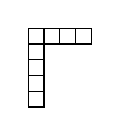
\begin{tikzpicture}
  \draw (0.00, 0.00) rectangle (0.20, -0.20);
  \draw (0.20, 0.00) rectangle (0.40, -0.20);
  \draw (0.40, 0.00) rectangle (0.60, -0.20);
  \draw (0.60, 0.00) rectangle (0.80, -0.20);
  \draw (0.00, -0.20) rectangle (0.20, -0.40);
  \draw (0.00, -0.40) rectangle (0.20, -0.60);
  \draw (0.00, -0.60) rectangle (0.20, -0.80);
  \draw (0.00, -0.80) rectangle (0.20, -1.00);
\end{tikzpicture}
\end{minipage}
\subsubsection*{Gap Poset}
\begin{minipage}{0.48\textwidth}
\begin{tikzpicture}
  \node[minimum size=0.5cm] (1) at (0.00,-2.00) {1};
  \node[minimum size=0.5cm] (2) at (2.00,-2.00) {2};
  \node[minimum size=0.5cm] (3) at (4.00,-2.00) {3};
  \node[minimum size=0.5cm] (4) at (0.00,0.00) {4};
  \node[draw, rectangle, minimum size=0.5cm] (8) at (2.00,0.00) {8};
  % Draw the cover relations
  \draw (8) -- (2);
  \draw (8) -- (3);
  \draw (8) -- (1);
\end{tikzpicture}
\end{minipage}
\subsubsection*{Void Poset}
\begin{minipage}{0.48\textwidth}

\begin{tikzpicture}
  \node[draw, rectangle, minimum size=0.5cm] (4) at (0.00,0.00) {4};
\end{tikzpicture}
\end{minipage}
\newpage\subsection{MinGens: [5, 6, 7, 8]}
\subsubsection*{Invariants}
\begin{minipage}{0.48\textwidth}
\begin{tabular}{|c|c|c|c|c|c|c|}
\toprule
g & F & m & ewt & t & \(|M|\) & \(|\lambda|\) \\
\midrule
5 & 9 & 5 & 4 & 1 & 0 & 9 \\
\bottomrule
\end{tabular}
\end{minipage}
\subsubsection*{Partition}
\begin{minipage}{0.48\textwidth}
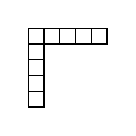
\begin{tikzpicture}
  \draw (0.00, 0.00) rectangle (0.20, -0.20);
  \draw (0.20, 0.00) rectangle (0.40, -0.20);
  \draw (0.40, 0.00) rectangle (0.60, -0.20);
  \draw (0.60, 0.00) rectangle (0.80, -0.20);
  \draw (0.80, 0.00) rectangle (1.00, -0.20);
  \draw (0.00, -0.20) rectangle (0.20, -0.40);
  \draw (0.00, -0.40) rectangle (0.20, -0.60);
  \draw (0.00, -0.60) rectangle (0.20, -0.80);
  \draw (0.00, -0.80) rectangle (0.20, -1.00);
\end{tikzpicture}
\end{minipage}
\subsubsection*{Gap Poset}
\begin{minipage}{0.48\textwidth}
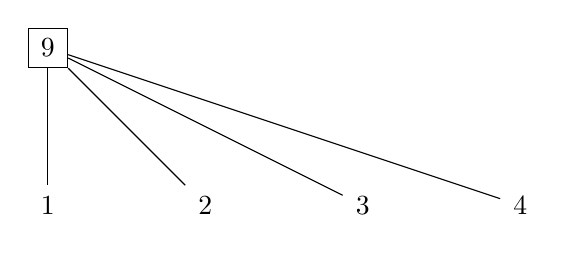
\begin{tikzpicture}
  \node[minimum size=0.5cm] (1) at (0.00,-2.00) {1};
  \node[minimum size=0.5cm] (2) at (2.00,-2.00) {2};
  \node[minimum size=0.5cm] (3) at (4.00,-2.00) {3};
  \node[minimum size=0.5cm] (4) at (6.00,-2.00) {4};
  \node[draw, rectangle, minimum size=0.5cm] (9) at (0.00,0.00) {9};
  % Draw the cover relations
  \draw (9) -- (1);
  \draw (9) -- (2);
  \draw (9) -- (3);
  \draw (9) -- (4);
\end{tikzpicture}
\end{minipage}
\subsubsection*{Void Poset}
\begin{minipage}{0.48\textwidth}
\end{minipage}
\newpage\subsection{MinGens: [4, 7, 9, 10]}
\subsubsection*{Invariants}
\begin{minipage}{0.48\textwidth}
\begin{tabular}{|c|c|c|c|c|c|c|}
\toprule
g & F & m & ewt & t & \(|M|\) & \(|\lambda|\) \\
\midrule
5 & 6 & 4 & 2 & 3 & 3 & 7 \\
\bottomrule
\end{tabular}
\end{minipage}
\subsubsection*{Partition}
\begin{minipage}{0.48\textwidth}
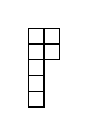
\begin{tikzpicture}
  \draw (0.00, 0.00) rectangle (0.20, -0.20);
  \draw (0.20, 0.00) rectangle (0.40, -0.20);
  \draw (0.00, -0.20) rectangle (0.20, -0.40);
  \draw (0.20, -0.20) rectangle (0.40, -0.40);
  \draw (0.00, -0.40) rectangle (0.20, -0.60);
  \draw (0.00, -0.60) rectangle (0.20, -0.80);
  \draw (0.00, -0.80) rectangle (0.20, -1.00);
\end{tikzpicture}
\end{minipage}
\subsubsection*{Gap Poset}
\begin{minipage}{0.48\textwidth}
\begin{tikzpicture}
  \node[minimum size=0.5cm] (1) at (0.00,-2.00) {1};
  \node[minimum size=0.5cm] (2) at (2.00,-2.00) {2};
  \node[minimum size=0.5cm] (3) at (0.00,0.00) {3};
  \node[minimum size=0.5cm] (5) at (2.00,0.00) {5};
  \node[draw, rectangle, minimum size=0.5cm] (6) at (4.00,0.00) {6};
  % Draw the cover relations
  \draw (6) -- (2);
  \draw (5) -- (1);
\end{tikzpicture}
\end{minipage}
\subsubsection*{Void Poset}
\begin{minipage}{0.48\textwidth}
\begin{tikzpicture}
  \node[minimum size=0.5cm] (1) at (0.00,-2.00) {1};
  \node[minimum size=0.5cm] (3) at (0.00,0.00) {3};
  \node[draw, rectangle, minimum size=0.5cm] (5) at (2.00,0.00) {5};
  % Draw the cover relations
  \draw (5) -- (1);
\end{tikzpicture}
\end{minipage}
\newpage\subsection{MinGens: [4, 6, 9, 11]}
\subsubsection*{Invariants}
\begin{minipage}{0.48\textwidth}
\begin{tabular}{|c|c|c|c|c|c|c|}
\toprule
g & F & m & ewt & t & \(|M|\) & \(|\lambda|\) \\
\midrule
5 & 7 & 4 & 3 & 3 & 2 & 8 \\
\bottomrule
\end{tabular}
\end{minipage}
\subsubsection*{Partition}
\begin{minipage}{0.48\textwidth}
\begin{tikzpicture}
  \draw (0.00, 0.00) rectangle (0.20, -0.20);
  \draw (0.20, 0.00) rectangle (0.40, -0.20);
  \draw (0.40, 0.00) rectangle (0.60, -0.20);
  \draw (0.00, -0.20) rectangle (0.20, -0.40);
  \draw (0.20, -0.20) rectangle (0.40, -0.40);
  \draw (0.00, -0.40) rectangle (0.20, -0.60);
  \draw (0.00, -0.60) rectangle (0.20, -0.80);
  \draw (0.00, -0.80) rectangle (0.20, -1.00);
\end{tikzpicture}
\end{minipage}
\subsubsection*{Gap Poset}
\begin{minipage}{0.48\textwidth}
\begin{tikzpicture}
  \node[minimum size=0.5cm] (1) at (0.00,-2.00) {1};
  \node[minimum size=0.5cm] (3) at (2.00,-2.00) {3};
  \node[minimum size=0.5cm] (2) at (0.00,0.00) {2};
  \node[minimum size=0.5cm] (5) at (2.00,0.00) {5};
  \node[draw, rectangle, minimum size=0.5cm] (7) at (4.00,0.00) {7};
  % Draw the cover relations
  \draw (7) -- (1);
  \draw (5) -- (1);
  \draw (7) -- (3);
\end{tikzpicture}
\end{minipage}
\subsubsection*{Void Poset}
\begin{minipage}{0.48\textwidth}
\begin{tikzpicture}
  \node[minimum size=0.5cm] (2) at (0.00,0.00) {2};
  \node[draw, rectangle, minimum size=0.5cm] (5) at (2.00,0.00) {5};
\end{tikzpicture}
\end{minipage}
\newpage\subsection{MinGens: [4, 6, 7]}
\subsubsection*{Invariants}
\begin{minipage}{0.48\textwidth}
\begin{tabular}{|c|c|c|c|c|c|c|}
\toprule
g & F & m & ewt & t & \(|M|\) & \(|\lambda|\) \\
\midrule
5 & 9 & 4 & 4 & 1 & 0 & 10 \\
\bottomrule
\end{tabular}
\end{minipage}
\subsubsection*{Partition}
\begin{minipage}{0.48\textwidth}
\begin{tikzpicture}
  \draw (0.00, 0.00) rectangle (0.20, -0.20);
  \draw (0.20, 0.00) rectangle (0.40, -0.20);
  \draw (0.40, 0.00) rectangle (0.60, -0.20);
  \draw (0.60, 0.00) rectangle (0.80, -0.20);
  \draw (0.80, 0.00) rectangle (1.00, -0.20);
  \draw (0.00, -0.20) rectangle (0.20, -0.40);
  \draw (0.20, -0.20) rectangle (0.40, -0.40);
  \draw (0.00, -0.40) rectangle (0.20, -0.60);
  \draw (0.00, -0.60) rectangle (0.20, -0.80);
  \draw (0.00, -0.80) rectangle (0.20, -1.00);
\end{tikzpicture}
\end{minipage}
\subsubsection*{Gap Poset}
\begin{minipage}{0.48\textwidth}
\begin{tikzpicture}
  \node[minimum size=0.5cm] (1) at (0.00,-4.00) {1};
  \node[minimum size=0.5cm] (2) at (0.00,-2.00) {2};
  \node[minimum size=0.5cm] (3) at (2.00,-2.00) {3};
  \node[minimum size=0.5cm] (5) at (4.00,-2.00) {5};
  \node[draw, rectangle, minimum size=0.5cm] (9) at (0.00,0.00) {9};
  % Draw the cover relations
  \draw (9) -- (5);
  \draw (9) -- (2);
  \draw (5) -- (1);
  \draw (9) -- (3);
\end{tikzpicture}
\end{minipage}
\subsubsection*{Void Poset}
\begin{minipage}{0.48\textwidth}
\end{minipage}
\newpage\subsection{MinGens: [4, 5, 11]}
\subsubsection*{Invariants}
\begin{minipage}{0.48\textwidth}
\begin{tabular}{|c|c|c|c|c|c|c|}
\toprule
g & F & m & ewt & t & \(|M|\) & \(|\lambda|\) \\
\midrule
5 & 7 & 4 & 4 & 2 & 2 & 9 \\
\bottomrule
\end{tabular}
\end{minipage}
\subsubsection*{Partition}
\begin{minipage}{0.48\textwidth}
\begin{tikzpicture}
  \draw (0.00, 0.00) rectangle (0.20, -0.20);
  \draw (0.20, 0.00) rectangle (0.40, -0.20);
  \draw (0.40, 0.00) rectangle (0.60, -0.20);
  \draw (0.00, -0.20) rectangle (0.20, -0.40);
  \draw (0.20, -0.20) rectangle (0.40, -0.40);
  \draw (0.40, -0.20) rectangle (0.60, -0.40);
  \draw (0.00, -0.40) rectangle (0.20, -0.60);
  \draw (0.00, -0.60) rectangle (0.20, -0.80);
  \draw (0.00, -0.80) rectangle (0.20, -1.00);
\end{tikzpicture}
\end{minipage}
\subsubsection*{Gap Poset}
\begin{minipage}{0.48\textwidth}
\begin{tikzpicture}
  \node[minimum size=0.5cm] (1) at (0.00,-2.00) {1};
  \node[minimum size=0.5cm] (2) at (2.00,-2.00) {2};
  \node[minimum size=0.5cm] (3) at (4.00,-2.00) {3};
  \node[minimum size=0.5cm] (6) at (0.00,0.00) {6};
  \node[draw, rectangle, minimum size=0.5cm] (7) at (2.00,0.00) {7};
  % Draw the cover relations
  \draw (6) -- (1);
  \draw (6) -- (2);
  \draw (7) -- (2);
  \draw (7) -- (3);
\end{tikzpicture}
\end{minipage}
\subsubsection*{Void Poset}
\begin{minipage}{0.48\textwidth}
\begin{tikzpicture}
  \node[minimum size=0.5cm] (1) at (0.00,-2.00) {1};
  \node[draw, rectangle, minimum size=0.5cm] (6) at (0.00,0.00) {6};
  % Draw the cover relations
  \draw (6) -- (1);
\end{tikzpicture}
\end{minipage}
\newpage\subsection{MinGens: [3, 8, 10]}
\subsubsection*{Invariants}
\begin{minipage}{0.48\textwidth}
\begin{tabular}{|c|c|c|c|c|c|c|}
\toprule
g & F & m & ewt & t & \(|M|\) & \(|\lambda|\) \\
\midrule
5 & 7 & 3 & 3 & 2 & 2 & 9 \\
\bottomrule
\end{tabular}
\end{minipage}
\subsubsection*{Partition}
\begin{minipage}{0.48\textwidth}
\begin{tikzpicture}
  \draw (0.00, 0.00) rectangle (0.20, -0.20);
  \draw (0.20, 0.00) rectangle (0.40, -0.20);
  \draw (0.40, 0.00) rectangle (0.60, -0.20);
  \draw (0.00, -0.20) rectangle (0.20, -0.40);
  \draw (0.20, -0.20) rectangle (0.40, -0.40);
  \draw (0.00, -0.40) rectangle (0.20, -0.60);
  \draw (0.20, -0.40) rectangle (0.40, -0.60);
  \draw (0.00, -0.60) rectangle (0.20, -0.80);
  \draw (0.00, -0.80) rectangle (0.20, -1.00);
\end{tikzpicture}
\end{minipage}
\subsubsection*{Gap Poset}
\begin{minipage}{0.48\textwidth}
\begin{tikzpicture}
  \node[minimum size=0.5cm] (1) at (0.00,-4.00) {1};
  \node[minimum size=0.5cm] (2) at (0.00,-2.00) {2};
  \node[minimum size=0.5cm] (4) at (2.00,-2.00) {4};
  \node[minimum size=0.5cm] (5) at (0.00,0.00) {5};
  \node[draw, rectangle, minimum size=0.5cm] (7) at (2.00,0.00) {7};
  % Draw the cover relations
  \draw (7) -- (4);
  \draw (4) -- (1);
  \draw (5) -- (2);
\end{tikzpicture}
\end{minipage}
\subsubsection*{Void Poset}
\begin{minipage}{0.48\textwidth}
\begin{tikzpicture}
  \node[minimum size=0.5cm] (2) at (0.00,-2.00) {2};
  \node[draw, rectangle, minimum size=0.5cm] (5) at (0.00,0.00) {5};
  % Draw the cover relations
  \draw (5) -- (2);
\end{tikzpicture}
\end{minipage}
\newpage\subsection{MinGens: [3, 7, 11]}
\subsubsection*{Invariants}
\begin{minipage}{0.48\textwidth}
\begin{tabular}{|c|c|c|c|c|c|c|}
\toprule
g & F & m & ewt & t & \(|M|\) & \(|\lambda|\) \\
\midrule
5 & 8 & 3 & 4 & 2 & 1 & 10 \\
\bottomrule
\end{tabular}
\end{minipage}
\subsubsection*{Partition}
\begin{minipage}{0.48\textwidth}
\begin{tikzpicture}
  \draw (0.00, 0.00) rectangle (0.20, -0.20);
  \draw (0.20, 0.00) rectangle (0.40, -0.20);
  \draw (0.40, 0.00) rectangle (0.60, -0.20);
  \draw (0.60, 0.00) rectangle (0.80, -0.20);
  \draw (0.00, -0.20) rectangle (0.20, -0.40);
  \draw (0.20, -0.20) rectangle (0.40, -0.40);
  \draw (0.00, -0.40) rectangle (0.20, -0.60);
  \draw (0.20, -0.40) rectangle (0.40, -0.60);
  \draw (0.00, -0.60) rectangle (0.20, -0.80);
  \draw (0.00, -0.80) rectangle (0.20, -1.00);
\end{tikzpicture}
\end{minipage}
\subsubsection*{Gap Poset}
\begin{minipage}{0.48\textwidth}
\begin{tikzpicture}
  \node[minimum size=0.5cm] (1) at (0.00,-2.00) {1};
  \node[minimum size=0.5cm] (5) at (2.00,-2.00) {5};
  \node[minimum size=0.5cm] (2) at (2.00,-4.00) {2};
  \node[minimum size=0.5cm] (4) at (0.00,0.00) {4};
  \node[draw, rectangle, minimum size=0.5cm] (8) at (2.00,0.00) {8};
  % Draw the cover relations
  \draw (5) -- (2);
  \draw (4) -- (1);
  \draw (8) -- (5);
  \draw (8) -- (1);
\end{tikzpicture}
\end{minipage}
\subsubsection*{Void Poset}
\begin{minipage}{0.48\textwidth}
\begin{tikzpicture}
  \node[draw, rectangle, minimum size=0.5cm] (4) at (0.00,0.00) {4};
\end{tikzpicture}
\end{minipage}
\newpage\subsection{MinGens: [2, 11]}
\subsubsection*{Invariants}
\begin{minipage}{0.48\textwidth}
\begin{tabular}{|c|c|c|c|c|c|c|}
\toprule
g & F & m & ewt & t & \(|M|\) & \(|\lambda|\) \\
\midrule
5 & 9 & 2 & 4 & 1 & 0 & 15 \\
\bottomrule
\end{tabular}
\end{minipage}
\subsubsection*{Partition}
\begin{minipage}{0.48\textwidth}
\begin{tikzpicture}
  \draw (0.00, 0.00) rectangle (0.20, -0.20);
  \draw (0.20, 0.00) rectangle (0.40, -0.20);
  \draw (0.40, 0.00) rectangle (0.60, -0.20);
  \draw (0.60, 0.00) rectangle (0.80, -0.20);
  \draw (0.80, 0.00) rectangle (1.00, -0.20);
  \draw (0.00, -0.20) rectangle (0.20, -0.40);
  \draw (0.20, -0.20) rectangle (0.40, -0.40);
  \draw (0.40, -0.20) rectangle (0.60, -0.40);
  \draw (0.60, -0.20) rectangle (0.80, -0.40);
  \draw (0.00, -0.40) rectangle (0.20, -0.60);
  \draw (0.20, -0.40) rectangle (0.40, -0.60);
  \draw (0.40, -0.40) rectangle (0.60, -0.60);
  \draw (0.00, -0.60) rectangle (0.20, -0.80);
  \draw (0.20, -0.60) rectangle (0.40, -0.80);
  \draw (0.00, -0.80) rectangle (0.20, -1.00);
\end{tikzpicture}
\end{minipage}
\subsubsection*{Gap Poset}
\begin{minipage}{0.48\textwidth}
\begin{tikzpicture}
  \node[minimum size=0.5cm] (1) at (0.00,-8.00) {1};
  \node[minimum size=0.5cm] (3) at (0.00,-6.00) {3};
  \node[minimum size=0.5cm] (5) at (0.00,-4.00) {5};
  \node[minimum size=0.5cm] (7) at (0.00,-2.00) {7};
  \node[draw, rectangle, minimum size=0.5cm] (9) at (0.00,0.00) {9};
  % Draw the cover relations
  \draw (3) -- (1);
  \draw (5) -- (3);
  \draw (9) -- (7);
  \draw (7) -- (5);
\end{tikzpicture}
\end{minipage}
\subsubsection*{Void Poset}
\begin{minipage}{0.48\textwidth}
\end{minipage}
\section{Genus 6}
\newpage\subsection{MinGens: [7, 8, 9, 10, 11, 12, 13]}
\subsubsection*{Invariants}
\begin{minipage}{0.48\textwidth}
\begin{tabular}{|c|c|c|c|c|c|c|}
\toprule
g & F & m & ewt & t & \(|M|\) & \(|\lambda|\) \\
\midrule
6 & 6 & 7 & 0 & 6 & 5 & 6 \\
\bottomrule
\end{tabular}
\end{minipage}
\subsubsection*{Partition}
\begin{minipage}{0.48\textwidth}
\begin{tikzpicture}
  \draw (0.00, 0.00) rectangle (0.20, -0.20);
  \draw (0.00, -0.20) rectangle (0.20, -0.40);
  \draw (0.00, -0.40) rectangle (0.20, -0.60);
  \draw (0.00, -0.60) rectangle (0.20, -0.80);
  \draw (0.00, -0.80) rectangle (0.20, -1.00);
  \draw (0.00, -1.00) rectangle (0.20, -1.20);
\end{tikzpicture}
\end{minipage}
\subsubsection*{Gap Poset}
\begin{minipage}{0.48\textwidth}
\begin{tikzpicture}
  \node[minimum size=0.5cm] (1) at (0.00,0.00) {1};
  \node[minimum size=0.5cm] (2) at (2.00,0.00) {2};
  \node[minimum size=0.5cm] (3) at (4.00,0.00) {3};
  \node[minimum size=0.5cm] (4) at (6.00,0.00) {4};
  \node[minimum size=0.5cm] (5) at (8.00,0.00) {5};
  \node[draw, rectangle, minimum size=0.5cm] (6) at (10.00,0.00) {6};
\end{tikzpicture}
\end{minipage}
\subsubsection*{Void Poset}
\begin{minipage}{0.48\textwidth}
\begin{tikzpicture}
  \node[minimum size=0.5cm] (1) at (0.00,0.00) {1};
  \node[minimum size=0.5cm] (2) at (2.00,0.00) {2};
  \node[minimum size=0.5cm] (3) at (4.00,0.00) {3};
  \node[minimum size=0.5cm] (4) at (6.00,0.00) {4};
  \node[draw, rectangle, minimum size=0.5cm] (5) at (8.00,0.00) {5};
\end{tikzpicture}
\end{minipage}
\newpage\subsection{MinGens: [6, 8, 9, 10, 11, 13]}
\subsubsection*{Invariants}
\begin{minipage}{0.48\textwidth}
\begin{tabular}{|c|c|c|c|c|c|c|}
\toprule
g & F & m & ewt & t & \(|M|\) & \(|\lambda|\) \\
\midrule
6 & 7 & 6 & 1 & 5 & 4 & 7 \\
\bottomrule
\end{tabular}
\end{minipage}
\subsubsection*{Partition}
\begin{minipage}{0.48\textwidth}
\begin{tikzpicture}
  \draw (0.00, 0.00) rectangle (0.20, -0.20);
  \draw (0.20, 0.00) rectangle (0.40, -0.20);
  \draw (0.00, -0.20) rectangle (0.20, -0.40);
  \draw (0.00, -0.40) rectangle (0.20, -0.60);
  \draw (0.00, -0.60) rectangle (0.20, -0.80);
  \draw (0.00, -0.80) rectangle (0.20, -1.00);
  \draw (0.00, -1.00) rectangle (0.20, -1.20);
\end{tikzpicture}
\end{minipage}
\subsubsection*{Gap Poset}
\begin{minipage}{0.48\textwidth}
\begin{tikzpicture}
  \node[minimum size=0.5cm] (1) at (0.00,-2.00) {1};
  \node[minimum size=0.5cm] (2) at (0.00,0.00) {2};
  \node[minimum size=0.5cm] (3) at (2.00,0.00) {3};
  \node[minimum size=0.5cm] (4) at (4.00,0.00) {4};
  \node[minimum size=0.5cm] (5) at (6.00,0.00) {5};
  \node[draw, rectangle, minimum size=0.5cm] (7) at (8.00,0.00) {7};
  % Draw the cover relations
  \draw (7) -- (1);
\end{tikzpicture}
\end{minipage}
\subsubsection*{Void Poset}
\begin{minipage}{0.48\textwidth}
\begin{tikzpicture}
  \node[minimum size=0.5cm] (2) at (0.00,0.00) {2};
  \node[minimum size=0.5cm] (3) at (2.00,0.00) {3};
  \node[minimum size=0.5cm] (4) at (4.00,0.00) {4};
  \node[draw, rectangle, minimum size=0.5cm] (5) at (6.00,0.00) {5};
\end{tikzpicture}
\end{minipage}
\newpage\subsection{MinGens: [6, 7, 9, 10, 11]}
\subsubsection*{Invariants}
\begin{minipage}{0.48\textwidth}
\begin{tabular}{|c|c|c|c|c|c|c|}
\toprule
g & F & m & ewt & t & \(|M|\) & \(|\lambda|\) \\
\midrule
6 & 8 & 6 & 2 & 4 & 3 & 8 \\
\bottomrule
\end{tabular}
\end{minipage}
\subsubsection*{Partition}
\begin{minipage}{0.48\textwidth}
\begin{tikzpicture}
  \draw (0.00, 0.00) rectangle (0.20, -0.20);
  \draw (0.20, 0.00) rectangle (0.40, -0.20);
  \draw (0.40, 0.00) rectangle (0.60, -0.20);
  \draw (0.00, -0.20) rectangle (0.20, -0.40);
  \draw (0.00, -0.40) rectangle (0.20, -0.60);
  \draw (0.00, -0.60) rectangle (0.20, -0.80);
  \draw (0.00, -0.80) rectangle (0.20, -1.00);
  \draw (0.00, -1.00) rectangle (0.20, -1.20);
\end{tikzpicture}
\end{minipage}
\subsubsection*{Gap Poset}
\begin{minipage}{0.48\textwidth}
\begin{tikzpicture}
  \node[minimum size=0.5cm] (1) at (0.00,-2.00) {1};
  \node[minimum size=0.5cm] (2) at (2.00,-2.00) {2};
  \node[minimum size=0.5cm] (3) at (0.00,0.00) {3};
  \node[minimum size=0.5cm] (4) at (2.00,0.00) {4};
  \node[minimum size=0.5cm] (5) at (4.00,0.00) {5};
  \node[draw, rectangle, minimum size=0.5cm] (8) at (6.00,0.00) {8};
  % Draw the cover relations
  \draw (8) -- (2);
  \draw (8) -- (1);
\end{tikzpicture}
\end{minipage}
\subsubsection*{Void Poset}
\begin{minipage}{0.48\textwidth}
\begin{tikzpicture}
  \node[minimum size=0.5cm] (3) at (0.00,0.00) {3};
  \node[minimum size=0.5cm] (4) at (2.00,0.00) {4};
  \node[draw, rectangle, minimum size=0.5cm] (5) at (4.00,0.00) {5};
\end{tikzpicture}
\end{minipage}
\newpage\subsection{MinGens: [6, 7, 8, 10, 11]}
\subsubsection*{Invariants}
\begin{minipage}{0.48\textwidth}
\begin{tabular}{|c|c|c|c|c|c|c|}
\toprule
g & F & m & ewt & t & \(|M|\) & \(|\lambda|\) \\
\midrule
6 & 9 & 6 & 3 & 3 & 2 & 9 \\
\bottomrule
\end{tabular}
\end{minipage}
\subsubsection*{Partition}
\begin{minipage}{0.48\textwidth}
\begin{tikzpicture}
  \draw (0.00, 0.00) rectangle (0.20, -0.20);
  \draw (0.20, 0.00) rectangle (0.40, -0.20);
  \draw (0.40, 0.00) rectangle (0.60, -0.20);
  \draw (0.60, 0.00) rectangle (0.80, -0.20);
  \draw (0.00, -0.20) rectangle (0.20, -0.40);
  \draw (0.00, -0.40) rectangle (0.20, -0.60);
  \draw (0.00, -0.60) rectangle (0.20, -0.80);
  \draw (0.00, -0.80) rectangle (0.20, -1.00);
  \draw (0.00, -1.00) rectangle (0.20, -1.20);
\end{tikzpicture}
\end{minipage}
\subsubsection*{Gap Poset}
\begin{minipage}{0.48\textwidth}
\begin{tikzpicture}
  \node[minimum size=0.5cm] (1) at (0.00,-2.00) {1};
  \node[minimum size=0.5cm] (2) at (2.00,-2.00) {2};
  \node[minimum size=0.5cm] (3) at (4.00,-2.00) {3};
  \node[minimum size=0.5cm] (4) at (0.00,0.00) {4};
  \node[minimum size=0.5cm] (5) at (2.00,0.00) {5};
  \node[draw, rectangle, minimum size=0.5cm] (9) at (4.00,0.00) {9};
  % Draw the cover relations
  \draw (9) -- (1);
  \draw (9) -- (2);
  \draw (9) -- (3);
\end{tikzpicture}
\end{minipage}
\subsubsection*{Void Poset}
\begin{minipage}{0.48\textwidth}
\begin{tikzpicture}
  \node[minimum size=0.5cm] (4) at (0.00,0.00) {4};
  \node[draw, rectangle, minimum size=0.5cm] (5) at (2.00,0.00) {5};
\end{tikzpicture}
\end{minipage}
\newpage\subsection{MinGens: [6, 7, 8, 9, 11]}
\subsubsection*{Invariants}
\begin{minipage}{0.48\textwidth}
\begin{tabular}{|c|c|c|c|c|c|c|}
\toprule
g & F & m & ewt & t & \(|M|\) & \(|\lambda|\) \\
\midrule
6 & 10 & 6 & 4 & 2 & 1 & 10 \\
\bottomrule
\end{tabular}
\end{minipage}
\subsubsection*{Partition}
\begin{minipage}{0.48\textwidth}
\begin{tikzpicture}
  \draw (0.00, 0.00) rectangle (0.20, -0.20);
  \draw (0.20, 0.00) rectangle (0.40, -0.20);
  \draw (0.40, 0.00) rectangle (0.60, -0.20);
  \draw (0.60, 0.00) rectangle (0.80, -0.20);
  \draw (0.80, 0.00) rectangle (1.00, -0.20);
  \draw (0.00, -0.20) rectangle (0.20, -0.40);
  \draw (0.00, -0.40) rectangle (0.20, -0.60);
  \draw (0.00, -0.60) rectangle (0.20, -0.80);
  \draw (0.00, -0.80) rectangle (0.20, -1.00);
  \draw (0.00, -1.00) rectangle (0.20, -1.20);
\end{tikzpicture}
\end{minipage}
\subsubsection*{Gap Poset}
\begin{minipage}{0.48\textwidth}
\begin{tikzpicture}
  \node[minimum size=0.5cm] (1) at (0.00,-2.00) {1};
  \node[minimum size=0.5cm] (2) at (2.00,-2.00) {2};
  \node[minimum size=0.5cm] (3) at (4.00,-2.00) {3};
  \node[minimum size=0.5cm] (4) at (6.00,-2.00) {4};
  \node[minimum size=0.5cm] (5) at (0.00,0.00) {5};
  \node[draw, rectangle, minimum size=0.5cm] (10) at (2.00,0.00) {10};
  % Draw the cover relations
  \draw (10) -- (4);
  \draw (10) -- (1);
  \draw (10) -- (2);
  \draw (10) -- (3);
\end{tikzpicture}
\end{minipage}
\subsubsection*{Void Poset}
\begin{minipage}{0.48\textwidth}
\begin{tikzpicture}
  \node[draw, rectangle, minimum size=0.5cm] (5) at (0.00,0.00) {5};
\end{tikzpicture}
\end{minipage}
\newpage\subsection{MinGens: [6, 7, 8, 9, 10]}
\subsubsection*{Invariants}
\begin{minipage}{0.48\textwidth}
\begin{tabular}{|c|c|c|c|c|c|c|}
\toprule
g & F & m & ewt & t & \(|M|\) & \(|\lambda|\) \\
\midrule
6 & 11 & 6 & 5 & 1 & 0 & 11 \\
\bottomrule
\end{tabular}
\end{minipage}
\subsubsection*{Partition}
\begin{minipage}{0.48\textwidth}
\begin{tikzpicture}
  \draw (0.00, 0.00) rectangle (0.20, -0.20);
  \draw (0.20, 0.00) rectangle (0.40, -0.20);
  \draw (0.40, 0.00) rectangle (0.60, -0.20);
  \draw (0.60, 0.00) rectangle (0.80, -0.20);
  \draw (0.80, 0.00) rectangle (1.00, -0.20);
  \draw (1.00, 0.00) rectangle (1.20, -0.20);
  \draw (0.00, -0.20) rectangle (0.20, -0.40);
  \draw (0.00, -0.40) rectangle (0.20, -0.60);
  \draw (0.00, -0.60) rectangle (0.20, -0.80);
  \draw (0.00, -0.80) rectangle (0.20, -1.00);
  \draw (0.00, -1.00) rectangle (0.20, -1.20);
\end{tikzpicture}
\end{minipage}
\subsubsection*{Gap Poset}
\begin{minipage}{0.48\textwidth}
\begin{tikzpicture}
  \node[minimum size=0.5cm] (1) at (0.00,-2.00) {1};
  \node[minimum size=0.5cm] (2) at (2.00,-2.00) {2};
  \node[minimum size=0.5cm] (3) at (4.00,-2.00) {3};
  \node[minimum size=0.5cm] (4) at (6.00,-2.00) {4};
  \node[minimum size=0.5cm] (5) at (8.00,-2.00) {5};
  \node[draw, rectangle, minimum size=0.5cm] (11) at (0.00,0.00) {11};
  % Draw the cover relations
  \draw (11) -- (1);
  \draw (11) -- (3);
  \draw (11) -- (2);
  \draw (11) -- (5);
  \draw (11) -- (4);
\end{tikzpicture}
\end{minipage}
\subsubsection*{Void Poset}
\begin{minipage}{0.48\textwidth}
\end{minipage}
\newpage\subsection{MinGens: [5, 8, 9, 11, 12]}
\subsubsection*{Invariants}
\begin{minipage}{0.48\textwidth}
\begin{tabular}{|c|c|c|c|c|c|c|}
\toprule
g & F & m & ewt & t & \(|M|\) & \(|\lambda|\) \\
\midrule
6 & 7 & 5 & 2 & 4 & 4 & 8 \\
\bottomrule
\end{tabular}
\end{minipage}
\subsubsection*{Partition}
\begin{minipage}{0.48\textwidth}
\begin{tikzpicture}
  \draw (0.00, 0.00) rectangle (0.20, -0.20);
  \draw (0.20, 0.00) rectangle (0.40, -0.20);
  \draw (0.00, -0.20) rectangle (0.20, -0.40);
  \draw (0.20, -0.20) rectangle (0.40, -0.40);
  \draw (0.00, -0.40) rectangle (0.20, -0.60);
  \draw (0.00, -0.60) rectangle (0.20, -0.80);
  \draw (0.00, -0.80) rectangle (0.20, -1.00);
  \draw (0.00, -1.00) rectangle (0.20, -1.20);
\end{tikzpicture}
\end{minipage}
\subsubsection*{Gap Poset}
\begin{minipage}{0.48\textwidth}
\begin{tikzpicture}
  \node[minimum size=0.5cm] (1) at (0.00,-2.00) {1};
  \node[minimum size=0.5cm] (2) at (2.00,-2.00) {2};
  \node[minimum size=0.5cm] (3) at (0.00,0.00) {3};
  \node[minimum size=0.5cm] (4) at (2.00,0.00) {4};
  \node[minimum size=0.5cm] (6) at (4.00,0.00) {6};
  \node[draw, rectangle, minimum size=0.5cm] (7) at (6.00,0.00) {7};
  % Draw the cover relations
  \draw (6) -- (1);
  \draw (7) -- (2);
\end{tikzpicture}
\end{minipage}
\subsubsection*{Void Poset}
\begin{minipage}{0.48\textwidth}
\begin{tikzpicture}
  \node[minimum size=0.5cm] (1) at (0.00,-2.00) {1};
  \node[minimum size=0.5cm] (3) at (0.00,0.00) {3};
  \node[minimum size=0.5cm] (4) at (2.00,0.00) {4};
  \node[draw, rectangle, minimum size=0.5cm] (6) at (4.00,0.00) {6};
  % Draw the cover relations
  \draw (6) -- (1);
\end{tikzpicture}
\end{minipage}
\newpage\subsection{MinGens: [5, 7, 9, 11, 13]}
\subsubsection*{Invariants}
\begin{minipage}{0.48\textwidth}
\begin{tabular}{|c|c|c|c|c|c|c|}
\toprule
g & F & m & ewt & t & \(|M|\) & \(|\lambda|\) \\
\midrule
6 & 8 & 5 & 3 & 4 & 3 & 9 \\
\bottomrule
\end{tabular}
\end{minipage}
\subsubsection*{Partition}
\begin{minipage}{0.48\textwidth}
\begin{tikzpicture}
  \draw (0.00, 0.00) rectangle (0.20, -0.20);
  \draw (0.20, 0.00) rectangle (0.40, -0.20);
  \draw (0.40, 0.00) rectangle (0.60, -0.20);
  \draw (0.00, -0.20) rectangle (0.20, -0.40);
  \draw (0.20, -0.20) rectangle (0.40, -0.40);
  \draw (0.00, -0.40) rectangle (0.20, -0.60);
  \draw (0.00, -0.60) rectangle (0.20, -0.80);
  \draw (0.00, -0.80) rectangle (0.20, -1.00);
  \draw (0.00, -1.00) rectangle (0.20, -1.20);
\end{tikzpicture}
\end{minipage}
\subsubsection*{Gap Poset}
\begin{minipage}{0.48\textwidth}
\begin{tikzpicture}
  \node[minimum size=0.5cm] (1) at (0.00,-2.00) {1};
  \node[minimum size=0.5cm] (3) at (2.00,-2.00) {3};
  \node[minimum size=0.5cm] (2) at (0.00,0.00) {2};
  \node[minimum size=0.5cm] (4) at (2.00,0.00) {4};
  \node[minimum size=0.5cm] (6) at (4.00,0.00) {6};
  \node[draw, rectangle, minimum size=0.5cm] (8) at (6.00,0.00) {8};
  % Draw the cover relations
  \draw (6) -- (1);
  \draw (8) -- (3);
  \draw (8) -- (1);
\end{tikzpicture}
\end{minipage}
\subsubsection*{Void Poset}
\begin{minipage}{0.48\textwidth}
\begin{tikzpicture}
  \node[minimum size=0.5cm] (2) at (0.00,0.00) {2};
  \node[minimum size=0.5cm] (4) at (2.00,0.00) {4};
  \node[draw, rectangle, minimum size=0.5cm] (6) at (4.00,0.00) {6};
\end{tikzpicture}
\end{minipage}
\newpage\subsection{MinGens: [5, 7, 8, 11]}
\subsubsection*{Invariants}
\begin{minipage}{0.48\textwidth}
\begin{tabular}{|c|c|c|c|c|c|c|}
\toprule
g & F & m & ewt & t & \(|M|\) & \(|\lambda|\) \\
\midrule
6 & 9 & 5 & 4 & 3 & 2 & 10 \\
\bottomrule
\end{tabular}
\end{minipage}
\subsubsection*{Partition}
\begin{minipage}{0.48\textwidth}
\begin{tikzpicture}
  \draw (0.00, 0.00) rectangle (0.20, -0.20);
  \draw (0.20, 0.00) rectangle (0.40, -0.20);
  \draw (0.40, 0.00) rectangle (0.60, -0.20);
  \draw (0.60, 0.00) rectangle (0.80, -0.20);
  \draw (0.00, -0.20) rectangle (0.20, -0.40);
  \draw (0.20, -0.20) rectangle (0.40, -0.40);
  \draw (0.00, -0.40) rectangle (0.20, -0.60);
  \draw (0.00, -0.60) rectangle (0.20, -0.80);
  \draw (0.00, -0.80) rectangle (0.20, -1.00);
  \draw (0.00, -1.00) rectangle (0.20, -1.20);
\end{tikzpicture}
\end{minipage}
\subsubsection*{Gap Poset}
\begin{minipage}{0.48\textwidth}
\begin{tikzpicture}
  \node[minimum size=0.5cm] (1) at (0.00,-2.00) {1};
  \node[minimum size=0.5cm] (2) at (2.00,-2.00) {2};
  \node[minimum size=0.5cm] (4) at (4.00,-2.00) {4};
  \node[minimum size=0.5cm] (3) at (0.00,0.00) {3};
  \node[minimum size=0.5cm] (6) at (2.00,0.00) {6};
  \node[draw, rectangle, minimum size=0.5cm] (9) at (4.00,0.00) {9};
  % Draw the cover relations
  \draw (6) -- (1);
  \draw (9) -- (1);
  \draw (9) -- (2);
  \draw (9) -- (4);
\end{tikzpicture}
\end{minipage}
\subsubsection*{Void Poset}
\begin{minipage}{0.48\textwidth}
\begin{tikzpicture}
  \node[minimum size=0.5cm] (3) at (0.00,0.00) {3};
  \node[draw, rectangle, minimum size=0.5cm] (6) at (2.00,0.00) {6};
\end{tikzpicture}
\end{minipage}
\newpage\subsection{MinGens: [5, 7, 8, 9]}
\subsubsection*{Invariants}
\begin{minipage}{0.48\textwidth}
\begin{tabular}{|c|c|c|c|c|c|c|}
\toprule
g & F & m & ewt & t & \(|M|\) & \(|\lambda|\) \\
\midrule
6 & 11 & 5 & 5 & 1 & 0 & 12 \\
\bottomrule
\end{tabular}
\end{minipage}
\subsubsection*{Partition}
\begin{minipage}{0.48\textwidth}
\begin{tikzpicture}
  \draw (0.00, 0.00) rectangle (0.20, -0.20);
  \draw (0.20, 0.00) rectangle (0.40, -0.20);
  \draw (0.40, 0.00) rectangle (0.60, -0.20);
  \draw (0.60, 0.00) rectangle (0.80, -0.20);
  \draw (0.80, 0.00) rectangle (1.00, -0.20);
  \draw (1.00, 0.00) rectangle (1.20, -0.20);
  \draw (0.00, -0.20) rectangle (0.20, -0.40);
  \draw (0.20, -0.20) rectangle (0.40, -0.40);
  \draw (0.00, -0.40) rectangle (0.20, -0.60);
  \draw (0.00, -0.60) rectangle (0.20, -0.80);
  \draw (0.00, -0.80) rectangle (0.20, -1.00);
  \draw (0.00, -1.00) rectangle (0.20, -1.20);
\end{tikzpicture}
\end{minipage}
\subsubsection*{Gap Poset}
\begin{minipage}{0.48\textwidth}
\begin{tikzpicture}
  \node[minimum size=0.5cm] (1) at (0.00,-4.00) {1};
  \node[minimum size=0.5cm] (2) at (0.00,-2.00) {2};
  \node[minimum size=0.5cm] (3) at (2.00,-2.00) {3};
  \node[minimum size=0.5cm] (4) at (4.00,-2.00) {4};
  \node[minimum size=0.5cm] (6) at (6.00,-2.00) {6};
  \node[draw, rectangle, minimum size=0.5cm] (11) at (0.00,0.00) {11};
  % Draw the cover relations
  \draw (6) -- (1);
  \draw (11) -- (3);
  \draw (11) -- (6);
  \draw (11) -- (2);
  \draw (11) -- (4);
\end{tikzpicture}
\end{minipage}
\subsubsection*{Void Poset}
\begin{minipage}{0.48\textwidth}
\end{minipage}
\newpage\subsection{MinGens: [5, 6, 9, 13]}
\subsubsection*{Invariants}
\begin{minipage}{0.48\textwidth}
\begin{tabular}{|c|c|c|c|c|c|c|}
\toprule
g & F & m & ewt & t & \(|M|\) & \(|\lambda|\) \\
\midrule
6 & 8 & 5 & 4 & 3 & 3 & 10 \\
\bottomrule
\end{tabular}
\end{minipage}
\subsubsection*{Partition}
\begin{minipage}{0.48\textwidth}
\begin{tikzpicture}
  \draw (0.00, 0.00) rectangle (0.20, -0.20);
  \draw (0.20, 0.00) rectangle (0.40, -0.20);
  \draw (0.40, 0.00) rectangle (0.60, -0.20);
  \draw (0.00, -0.20) rectangle (0.20, -0.40);
  \draw (0.20, -0.20) rectangle (0.40, -0.40);
  \draw (0.40, -0.20) rectangle (0.60, -0.40);
  \draw (0.00, -0.40) rectangle (0.20, -0.60);
  \draw (0.00, -0.60) rectangle (0.20, -0.80);
  \draw (0.00, -0.80) rectangle (0.20, -1.00);
  \draw (0.00, -1.00) rectangle (0.20, -1.20);
\end{tikzpicture}
\end{minipage}
\subsubsection*{Gap Poset}
\begin{minipage}{0.48\textwidth}
\begin{tikzpicture}
  \node[minimum size=0.5cm] (1) at (0.00,-2.00) {1};
  \node[minimum size=0.5cm] (2) at (2.00,-2.00) {2};
  \node[minimum size=0.5cm] (3) at (4.00,-2.00) {3};
  \node[minimum size=0.5cm] (4) at (0.00,0.00) {4};
  \node[minimum size=0.5cm] (7) at (2.00,0.00) {7};
  \node[draw, rectangle, minimum size=0.5cm] (8) at (4.00,0.00) {8};
  % Draw the cover relations
  \draw (8) -- (2);
  \draw (8) -- (3);
  \draw (7) -- (1);
  \draw (7) -- (2);
\end{tikzpicture}
\end{minipage}
\subsubsection*{Void Poset}
\begin{minipage}{0.48\textwidth}
\begin{tikzpicture}
  \node[minimum size=0.5cm] (1) at (0.00,-2.00) {1};
  \node[minimum size=0.5cm] (4) at (0.00,0.00) {4};
  \node[draw, rectangle, minimum size=0.5cm] (7) at (2.00,0.00) {7};
  % Draw the cover relations
  \draw (7) -- (1);
\end{tikzpicture}
\end{minipage}
\newpage\subsection{MinGens: [5, 6, 8]}
\subsubsection*{Invariants}
\begin{minipage}{0.48\textwidth}
\begin{tabular}{|c|c|c|c|c|c|c|}
\toprule
g & F & m & ewt & t & \(|M|\) & \(|\lambda|\) \\
\midrule
6 & 9 & 5 & 5 & 2 & 2 & 11 \\
\bottomrule
\end{tabular}
\end{minipage}
\subsubsection*{Partition}
\begin{minipage}{0.48\textwidth}
\begin{tikzpicture}
  \draw (0.00, 0.00) rectangle (0.20, -0.20);
  \draw (0.20, 0.00) rectangle (0.40, -0.20);
  \draw (0.40, 0.00) rectangle (0.60, -0.20);
  \draw (0.60, 0.00) rectangle (0.80, -0.20);
  \draw (0.00, -0.20) rectangle (0.20, -0.40);
  \draw (0.20, -0.20) rectangle (0.40, -0.40);
  \draw (0.40, -0.20) rectangle (0.60, -0.40);
  \draw (0.00, -0.40) rectangle (0.20, -0.60);
  \draw (0.00, -0.60) rectangle (0.20, -0.80);
  \draw (0.00, -0.80) rectangle (0.20, -1.00);
  \draw (0.00, -1.00) rectangle (0.20, -1.20);
\end{tikzpicture}
\end{minipage}
\subsubsection*{Gap Poset}
\begin{minipage}{0.48\textwidth}
\begin{tikzpicture}
  \node[minimum size=0.5cm] (1) at (0.00,-2.00) {1};
  \node[minimum size=0.5cm] (2) at (2.00,-2.00) {2};
  \node[minimum size=0.5cm] (3) at (4.00,-2.00) {3};
  \node[minimum size=0.5cm] (4) at (6.00,-2.00) {4};
  \node[minimum size=0.5cm] (7) at (0.00,0.00) {7};
  \node[draw, rectangle, minimum size=0.5cm] (9) at (2.00,0.00) {9};
  % Draw the cover relations
  \draw (7) -- (1);
  \draw (9) -- (3);
  \draw (7) -- (2);
  \draw (9) -- (1);
  \draw (9) -- (4);
\end{tikzpicture}
\end{minipage}
\subsubsection*{Void Poset}
\begin{minipage}{0.48\textwidth}
\begin{tikzpicture}
  \node[minimum size=0.5cm] (2) at (0.00,-2.00) {2};
  \node[draw, rectangle, minimum size=0.5cm] (7) at (0.00,0.00) {7};
  % Draw the cover relations
  \draw (7) -- (2);
\end{tikzpicture}
\end{minipage}
\newpage\subsection{MinGens: [5, 6, 7]}
\subsubsection*{Invariants}
\begin{minipage}{0.48\textwidth}
\begin{tabular}{|c|c|c|c|c|c|c|}
\toprule
g & F & m & ewt & t & \(|M|\) & \(|\lambda|\) \\
\midrule
6 & 9 & 5 & 6 & 2 & 2 & 12 \\
\bottomrule
\end{tabular}
\end{minipage}
\subsubsection*{Partition}
\begin{minipage}{0.48\textwidth}
\begin{tikzpicture}
  \draw (0.00, 0.00) rectangle (0.20, -0.20);
  \draw (0.20, 0.00) rectangle (0.40, -0.20);
  \draw (0.40, 0.00) rectangle (0.60, -0.20);
  \draw (0.60, 0.00) rectangle (0.80, -0.20);
  \draw (0.00, -0.20) rectangle (0.20, -0.40);
  \draw (0.20, -0.20) rectangle (0.40, -0.40);
  \draw (0.40, -0.20) rectangle (0.60, -0.40);
  \draw (0.60, -0.20) rectangle (0.80, -0.40);
  \draw (0.00, -0.40) rectangle (0.20, -0.60);
  \draw (0.00, -0.60) rectangle (0.20, -0.80);
  \draw (0.00, -0.80) rectangle (0.20, -1.00);
  \draw (0.00, -1.00) rectangle (0.20, -1.20);
\end{tikzpicture}
\end{minipage}
\subsubsection*{Gap Poset}
\begin{minipage}{0.48\textwidth}
\begin{tikzpicture}
  \node[minimum size=0.5cm] (1) at (0.00,-2.00) {1};
  \node[minimum size=0.5cm] (2) at (2.00,-2.00) {2};
  \node[minimum size=0.5cm] (3) at (4.00,-2.00) {3};
  \node[minimum size=0.5cm] (4) at (6.00,-2.00) {4};
  \node[minimum size=0.5cm] (8) at (0.00,0.00) {8};
  \node[draw, rectangle, minimum size=0.5cm] (9) at (2.00,0.00) {9};
  % Draw the cover relations
  \draw (9) -- (3);
  \draw (8) -- (1);
  \draw (9) -- (2);
  \draw (8) -- (3);
  \draw (8) -- (2);
  \draw (9) -- (4);
\end{tikzpicture}
\end{minipage}
\subsubsection*{Void Poset}
\begin{minipage}{0.48\textwidth}
\begin{tikzpicture}
  \node[draw, rectangle, minimum size=0.5cm] (8) at (0.00,0.00) {8};
  \node[minimum size=0.5cm] (1) at (0.00,-2.00) {1};
  % Draw the cover relations
  \draw (8) -- (1);
\end{tikzpicture}
\end{minipage}
\newpage\subsection{MinGens: [4, 9, 10, 11]}
\subsubsection*{Invariants}
\begin{minipage}{0.48\textwidth}
\begin{tabular}{|c|c|c|c|c|c|c|}
\toprule
g & F & m & ewt & t & \(|M|\) & \(|\lambda|\) \\
\midrule
6 & 7 & 4 & 3 & 3 & 4 & 9 \\
\bottomrule
\end{tabular}
\end{minipage}
\subsubsection*{Partition}
\begin{minipage}{0.48\textwidth}
\begin{tikzpicture}
  \draw (0.00, 0.00) rectangle (0.20, -0.20);
  \draw (0.20, 0.00) rectangle (0.40, -0.20);
  \draw (0.00, -0.20) rectangle (0.20, -0.40);
  \draw (0.20, -0.20) rectangle (0.40, -0.40);
  \draw (0.00, -0.40) rectangle (0.20, -0.60);
  \draw (0.20, -0.40) rectangle (0.40, -0.60);
  \draw (0.00, -0.60) rectangle (0.20, -0.80);
  \draw (0.00, -0.80) rectangle (0.20, -1.00);
  \draw (0.00, -1.00) rectangle (0.20, -1.20);
\end{tikzpicture}
\end{minipage}
\subsubsection*{Gap Poset}
\begin{minipage}{0.48\textwidth}
\begin{tikzpicture}
  \node[minimum size=0.5cm] (1) at (0.00,-2.00) {1};
  \node[minimum size=0.5cm] (2) at (2.00,-2.00) {2};
  \node[minimum size=0.5cm] (3) at (4.00,-2.00) {3};
  \node[minimum size=0.5cm] (5) at (0.00,0.00) {5};
  \node[minimum size=0.5cm] (6) at (2.00,0.00) {6};
  \node[draw, rectangle, minimum size=0.5cm] (7) at (4.00,0.00) {7};
  % Draw the cover relations
  \draw (6) -- (2);
  \draw (5) -- (1);
  \draw (7) -- (3);
\end{tikzpicture}
\end{minipage}
\subsubsection*{Void Poset}
\begin{minipage}{0.48\textwidth}
\begin{tikzpicture}
  \node[minimum size=0.5cm] (1) at (0.00,-2.00) {1};
  \node[minimum size=0.5cm] (2) at (2.00,-2.00) {2};
  \node[minimum size=0.5cm] (5) at (0.00,0.00) {5};
  \node[draw, rectangle, minimum size=0.5cm] (6) at (2.00,0.00) {6};
  % Draw the cover relations
  \draw (6) -- (2);
  \draw (5) -- (1);
\end{tikzpicture}
\end{minipage}
\newpage\subsection{MinGens: [4, 7, 10, 13]}
\subsubsection*{Invariants}
\begin{minipage}{0.48\textwidth}
\begin{tabular}{|c|c|c|c|c|c|c|}
\toprule
g & F & m & ewt & t & \(|M|\) & \(|\lambda|\) \\
\midrule
6 & 9 & 4 & 4 & 3 & 2 & 11 \\
\bottomrule
\end{tabular}
\end{minipage}
\subsubsection*{Partition}
\begin{minipage}{0.48\textwidth}
\begin{tikzpicture}
  \draw (0.00, 0.00) rectangle (0.20, -0.20);
  \draw (0.20, 0.00) rectangle (0.40, -0.20);
  \draw (0.40, 0.00) rectangle (0.60, -0.20);
  \draw (0.60, 0.00) rectangle (0.80, -0.20);
  \draw (0.00, -0.20) rectangle (0.20, -0.40);
  \draw (0.20, -0.20) rectangle (0.40, -0.40);
  \draw (0.00, -0.40) rectangle (0.20, -0.60);
  \draw (0.20, -0.40) rectangle (0.40, -0.60);
  \draw (0.00, -0.60) rectangle (0.20, -0.80);
  \draw (0.00, -0.80) rectangle (0.20, -1.00);
  \draw (0.00, -1.00) rectangle (0.20, -1.20);
\end{tikzpicture}
\end{minipage}
\subsubsection*{Gap Poset}
\begin{minipage}{0.48\textwidth}
\begin{tikzpicture}
  \node[minimum size=0.5cm] (1) at (0.00,-4.00) {1};
  \node[minimum size=0.5cm] (2) at (0.00,-2.00) {2};
  \node[minimum size=0.5cm] (5) at (2.00,-2.00) {5};
  \node[minimum size=0.5cm] (3) at (0.00,0.00) {3};
  \node[minimum size=0.5cm] (6) at (2.00,0.00) {6};
  \node[draw, rectangle, minimum size=0.5cm] (9) at (4.00,0.00) {9};
  % Draw the cover relations
  \draw (9) -- (5);
  \draw (6) -- (2);
  \draw (5) -- (1);
  \draw (9) -- (2);
\end{tikzpicture}
\end{minipage}
\subsubsection*{Void Poset}
\begin{minipage}{0.48\textwidth}
\begin{tikzpicture}
  \node[minimum size=0.5cm] (3) at (0.00,0.00) {3};
  \node[draw, rectangle, minimum size=0.5cm] (6) at (2.00,0.00) {6};
\end{tikzpicture}
\end{minipage}
\newpage\subsection{MinGens: [4, 7, 9]}
\subsubsection*{Invariants}
\begin{minipage}{0.48\textwidth}
\begin{tabular}{|c|c|c|c|c|c|c|}
\toprule
g & F & m & ewt & t & \(|M|\) & \(|\lambda|\) \\
\midrule
6 & 10 & 4 & 5 & 2 & 1 & 12 \\
\bottomrule
\end{tabular}
\end{minipage}
\subsubsection*{Partition}
\begin{minipage}{0.48\textwidth}
\begin{tikzpicture}
  \draw (0.00, 0.00) rectangle (0.20, -0.20);
  \draw (0.20, 0.00) rectangle (0.40, -0.20);
  \draw (0.40, 0.00) rectangle (0.60, -0.20);
  \draw (0.60, 0.00) rectangle (0.80, -0.20);
  \draw (0.80, 0.00) rectangle (1.00, -0.20);
  \draw (0.00, -0.20) rectangle (0.20, -0.40);
  \draw (0.20, -0.20) rectangle (0.40, -0.40);
  \draw (0.00, -0.40) rectangle (0.20, -0.60);
  \draw (0.20, -0.40) rectangle (0.40, -0.60);
  \draw (0.00, -0.60) rectangle (0.20, -0.80);
  \draw (0.00, -0.80) rectangle (0.20, -1.00);
  \draw (0.00, -1.00) rectangle (0.20, -1.20);
\end{tikzpicture}
\end{minipage}
\subsubsection*{Gap Poset}
\begin{minipage}{0.48\textwidth}
\begin{tikzpicture}
  \node[minimum size=0.5cm] (1) at (0.00,-2.00) {1};
  \node[minimum size=0.5cm] (3) at (2.00,-2.00) {3};
  \node[minimum size=0.5cm] (6) at (4.00,-2.00) {6};
  \node[minimum size=0.5cm] (2) at (4.00,-4.00) {2};
  \node[minimum size=0.5cm] (5) at (0.00,0.00) {5};
  \node[draw, rectangle, minimum size=0.5cm] (10) at (2.00,0.00) {10};
  % Draw the cover relations
  \draw (6) -- (2);
  \draw (10) -- (1);
  \draw (5) -- (1);
  \draw (10) -- (6);
  \draw (10) -- (3);
\end{tikzpicture}
\end{minipage}
\subsubsection*{Void Poset}
\begin{minipage}{0.48\textwidth}
\begin{tikzpicture}
  \node[draw, rectangle, minimum size=0.5cm] (5) at (0.00,0.00) {5};
\end{tikzpicture}
\end{minipage}
\newpage\subsection{MinGens: [4, 6, 11, 13]}
\subsubsection*{Invariants}
\begin{minipage}{0.48\textwidth}
\begin{tabular}{|c|c|c|c|c|c|c|}
\toprule
g & F & m & ewt & t & \(|M|\) & \(|\lambda|\) \\
\midrule
6 & 9 & 4 & 5 & 3 & 2 & 12 \\
\bottomrule
\end{tabular}
\end{minipage}
\subsubsection*{Partition}
\begin{minipage}{0.48\textwidth}
\begin{tikzpicture}
  \draw (0.00, 0.00) rectangle (0.20, -0.20);
  \draw (0.20, 0.00) rectangle (0.40, -0.20);
  \draw (0.40, 0.00) rectangle (0.60, -0.20);
  \draw (0.60, 0.00) rectangle (0.80, -0.20);
  \draw (0.00, -0.20) rectangle (0.20, -0.40);
  \draw (0.20, -0.20) rectangle (0.40, -0.40);
  \draw (0.40, -0.20) rectangle (0.60, -0.40);
  \draw (0.00, -0.40) rectangle (0.20, -0.60);
  \draw (0.20, -0.40) rectangle (0.40, -0.60);
  \draw (0.00, -0.60) rectangle (0.20, -0.80);
  \draw (0.00, -0.80) rectangle (0.20, -1.00);
  \draw (0.00, -1.00) rectangle (0.20, -1.20);
\end{tikzpicture}
\end{minipage}
\subsubsection*{Gap Poset}
\begin{minipage}{0.48\textwidth}
\begin{tikzpicture}
  \node[minimum size=0.5cm] (1) at (0.00,-4.00) {1};
  \node[minimum size=0.5cm] (2) at (0.00,0.00) {2};
  \node[minimum size=0.5cm] (7) at (2.00,0.00) {7};
  \node[draw, rectangle, minimum size=0.5cm] (9) at (4.00,0.00) {9};
  \node[minimum size=0.5cm] (3) at (0.00,-2.00) {3};
  \node[minimum size=0.5cm] (5) at (2.00,-2.00) {5};
  % Draw the cover relations
  \draw (7) -- (1);
  \draw (9) -- (3);
  \draw (5) -- (1);
  \draw (7) -- (3);
  \draw (9) -- (5);
\end{tikzpicture}
\end{minipage}
\subsubsection*{Void Poset}
\begin{minipage}{0.48\textwidth}
\begin{tikzpicture}
  \node[minimum size=0.5cm] (2) at (0.00,0.00) {2};
  \node[draw, rectangle, minimum size=0.5cm] (7) at (2.00,0.00) {7};
\end{tikzpicture}
\end{minipage}
\newpage\subsection{MinGens: [4, 6, 9]}
\subsubsection*{Invariants}
\begin{minipage}{0.48\textwidth}
\begin{tabular}{|c|c|c|c|c|c|c|}
\toprule
g & F & m & ewt & t & \(|M|\) & \(|\lambda|\) \\
\midrule
6 & 11 & 4 & 6 & 1 & 0 & 14 \\
\bottomrule
\end{tabular}
\end{minipage}
\subsubsection*{Partition}
\begin{minipage}{0.48\textwidth}
\begin{tikzpicture}
  \draw (0.00, 0.00) rectangle (0.20, -0.20);
  \draw (0.20, 0.00) rectangle (0.40, -0.20);
  \draw (0.40, 0.00) rectangle (0.60, -0.20);
  \draw (0.60, 0.00) rectangle (0.80, -0.20);
  \draw (0.80, 0.00) rectangle (1.00, -0.20);
  \draw (1.00, 0.00) rectangle (1.20, -0.20);
  \draw (0.00, -0.20) rectangle (0.20, -0.40);
  \draw (0.20, -0.20) rectangle (0.40, -0.40);
  \draw (0.40, -0.20) rectangle (0.60, -0.40);
  \draw (0.00, -0.40) rectangle (0.20, -0.60);
  \draw (0.20, -0.40) rectangle (0.40, -0.60);
  \draw (0.00, -0.60) rectangle (0.20, -0.80);
  \draw (0.00, -0.80) rectangle (0.20, -1.00);
  \draw (0.00, -1.00) rectangle (0.20, -1.20);
\end{tikzpicture}
\end{minipage}
\subsubsection*{Gap Poset}
\begin{minipage}{0.48\textwidth}
\begin{tikzpicture}
  \node[minimum size=0.5cm] (1) at (0.00,-4.00) {1};
  \node[minimum size=0.5cm] (3) at (2.00,-4.00) {3};
  \node[minimum size=0.5cm] (2) at (0.00,-2.00) {2};
  \node[minimum size=0.5cm] (5) at (2.00,-2.00) {5};
  \node[minimum size=0.5cm] (7) at (4.00,-2.00) {7};
  \node[draw, rectangle, minimum size=0.5cm] (11) at (0.00,0.00) {11};
  % Draw the cover relations
  \draw (11) -- (7);
  \draw (7) -- (1);
  \draw (5) -- (1);
  \draw (7) -- (3);
  \draw (11) -- (2);
  \draw (11) -- (5);
\end{tikzpicture}
\end{minipage}
\subsubsection*{Void Poset}
\begin{minipage}{0.48\textwidth}
\end{minipage}
\newpage\subsection{MinGens: [4, 5]}
\subsubsection*{Invariants}
\begin{minipage}{0.48\textwidth}
\begin{tabular}{|c|c|c|c|c|c|c|}
\toprule
g & F & m & ewt & t & \(|M|\) & \(|\lambda|\) \\
\midrule
6 & 11 & 4 & 6 & 1 & 0 & 15 \\
\bottomrule
\end{tabular}
\end{minipage}
\subsubsection*{Partition}
\begin{minipage}{0.48\textwidth}
\begin{tikzpicture}
  \draw (0.00, 0.00) rectangle (0.20, -0.20);
  \draw (0.20, 0.00) rectangle (0.40, -0.20);
  \draw (0.40, 0.00) rectangle (0.60, -0.20);
  \draw (0.60, 0.00) rectangle (0.80, -0.20);
  \draw (0.80, 0.00) rectangle (1.00, -0.20);
  \draw (1.00, 0.00) rectangle (1.20, -0.20);
  \draw (0.00, -0.20) rectangle (0.20, -0.40);
  \draw (0.20, -0.20) rectangle (0.40, -0.40);
  \draw (0.40, -0.20) rectangle (0.60, -0.40);
  \draw (0.00, -0.40) rectangle (0.20, -0.60);
  \draw (0.20, -0.40) rectangle (0.40, -0.60);
  \draw (0.40, -0.40) rectangle (0.60, -0.60);
  \draw (0.00, -0.60) rectangle (0.20, -0.80);
  \draw (0.00, -0.80) rectangle (0.20, -1.00);
  \draw (0.00, -1.00) rectangle (0.20, -1.20);
\end{tikzpicture}
\end{minipage}
\subsubsection*{Gap Poset}
\begin{minipage}{0.48\textwidth}
\begin{tikzpicture}
  \node[minimum size=0.5cm] (1) at (0.00,-4.00) {1};
  \node[minimum size=0.5cm] (2) at (2.00,-4.00) {2};
  \node[minimum size=0.5cm] (3) at (4.00,-4.00) {3};
  \node[minimum size=0.5cm] (6) at (0.00,-2.00) {6};
  \node[minimum size=0.5cm] (7) at (2.00,-2.00) {7};
  \node[draw, rectangle, minimum size=0.5cm] (11) at (0.00,0.00) {11};
  % Draw the cover relations
  \draw (11) -- (7);
  \draw (6) -- (2);
  \draw (6) -- (1);
  \draw (11) -- (6);
  \draw (7) -- (3);
  \draw (7) -- (2);
\end{tikzpicture}
\end{minipage}
\subsubsection*{Void Poset}
\begin{minipage}{0.48\textwidth}
\end{minipage}
\newpage\subsection{MinGens: [3, 10, 11]}
\subsubsection*{Invariants}
\begin{minipage}{0.48\textwidth}
\begin{tabular}{|c|c|c|c|c|c|c|}
\toprule
g & F & m & ewt & t & \(|M|\) & \(|\lambda|\) \\
\midrule
6 & 8 & 3 & 4 & 2 & 3 & 12 \\
\bottomrule
\end{tabular}
\end{minipage}
\subsubsection*{Partition}
\begin{minipage}{0.48\textwidth}
\begin{tikzpicture}
  \draw (0.00, 0.00) rectangle (0.20, -0.20);
  \draw (0.20, 0.00) rectangle (0.40, -0.20);
  \draw (0.40, 0.00) rectangle (0.60, -0.20);
  \draw (0.00, -0.20) rectangle (0.20, -0.40);
  \draw (0.20, -0.20) rectangle (0.40, -0.40);
  \draw (0.40, -0.20) rectangle (0.60, -0.40);
  \draw (0.00, -0.40) rectangle (0.20, -0.60);
  \draw (0.20, -0.40) rectangle (0.40, -0.60);
  \draw (0.00, -0.60) rectangle (0.20, -0.80);
  \draw (0.20, -0.60) rectangle (0.40, -0.80);
  \draw (0.00, -0.80) rectangle (0.20, -1.00);
  \draw (0.00, -1.00) rectangle (0.20, -1.20);
\end{tikzpicture}
\end{minipage}
\subsubsection*{Gap Poset}
\begin{minipage}{0.48\textwidth}
\begin{tikzpicture}
  \node[minimum size=0.5cm] (1) at (0.00,-4.00) {1};
  \node[minimum size=0.5cm] (2) at (2.00,-4.00) {2};
  \node[minimum size=0.5cm] (4) at (0.00,-2.00) {4};
  \node[minimum size=0.5cm] (5) at (2.00,-2.00) {5};
  \node[minimum size=0.5cm] (7) at (0.00,0.00) {7};
  \node[draw, rectangle, minimum size=0.5cm] (8) at (2.00,0.00) {8};
  % Draw the cover relations
  \draw (7) -- (4);
  \draw (4) -- (1);
  \draw (8) -- (5);
  \draw (5) -- (2);
\end{tikzpicture}
\end{minipage}
\subsubsection*{Void Poset}
\begin{minipage}{0.48\textwidth}
\begin{tikzpicture}
  \node[minimum size=0.5cm] (1) at (0.00,-4.00) {1};
  \node[minimum size=0.5cm] (4) at (0.00,-2.00) {4};
  \node[draw, rectangle, minimum size=0.5cm] (7) at (0.00,0.00) {7};
  % Draw the cover relations
  \draw (7) -- (4);
  \draw (4) -- (1);
\end{tikzpicture}
\end{minipage}
\newpage\subsection{MinGens: [3, 8, 13]}
\subsubsection*{Invariants}
\begin{minipage}{0.48\textwidth}
\begin{tabular}{|c|c|c|c|c|c|c|}
\toprule
g & F & m & ewt & t & \(|M|\) & \(|\lambda|\) \\
\midrule
6 & 10 & 3 & 5 & 2 & 1 & 14 \\
\bottomrule
\end{tabular}
\end{minipage}
\subsubsection*{Partition}
\begin{minipage}{0.48\textwidth}
\begin{tikzpicture}
  \draw (0.00, 0.00) rectangle (0.20, -0.20);
  \draw (0.20, 0.00) rectangle (0.40, -0.20);
  \draw (0.40, 0.00) rectangle (0.60, -0.20);
  \draw (0.60, 0.00) rectangle (0.80, -0.20);
  \draw (0.80, 0.00) rectangle (1.00, -0.20);
  \draw (0.00, -0.20) rectangle (0.20, -0.40);
  \draw (0.20, -0.20) rectangle (0.40, -0.40);
  \draw (0.40, -0.20) rectangle (0.60, -0.40);
  \draw (0.00, -0.40) rectangle (0.20, -0.60);
  \draw (0.20, -0.40) rectangle (0.40, -0.60);
  \draw (0.00, -0.60) rectangle (0.20, -0.80);
  \draw (0.20, -0.60) rectangle (0.40, -0.80);
  \draw (0.00, -0.80) rectangle (0.20, -1.00);
  \draw (0.00, -1.00) rectangle (0.20, -1.20);
\end{tikzpicture}
\end{minipage}
\subsubsection*{Gap Poset}
\begin{minipage}{0.48\textwidth}
\begin{tikzpicture}
  \node[minimum size=0.5cm] (1) at (0.00,-6.00) {1};
  \node[minimum size=0.5cm] (2) at (0.00,-2.00) {2};
  \node[minimum size=0.5cm] (7) at (2.00,-2.00) {7};
  \node[minimum size=0.5cm] (4) at (2.00,-4.00) {4};
  \node[minimum size=0.5cm] (5) at (0.00,0.00) {5};
  \node[draw, rectangle, minimum size=0.5cm] (10) at (2.00,0.00) {10};
  % Draw the cover relations
  \draw (7) -- (4);
  \draw (10) -- (7);
  \draw (4) -- (1);
  \draw (10) -- (2);
  \draw (5) -- (2);
\end{tikzpicture}
\end{minipage}
\subsubsection*{Void Poset}
\begin{minipage}{0.48\textwidth}
\begin{tikzpicture}
  \node[draw, rectangle, minimum size=0.5cm] (5) at (0.00,0.00) {5};
\end{tikzpicture}
\end{minipage}
\newpage\subsection{MinGens: [3, 7]}
\subsubsection*{Invariants}
\begin{minipage}{0.48\textwidth}
\begin{tabular}{|c|c|c|c|c|c|c|}
\toprule
g & F & m & ewt & t & \(|M|\) & \(|\lambda|\) \\
\midrule
6 & 11 & 3 & 6 & 1 & 0 & 16 \\
\bottomrule
\end{tabular}
\end{minipage}
\subsubsection*{Partition}
\begin{minipage}{0.48\textwidth}
\begin{tikzpicture}
  \draw (0.00, 0.00) rectangle (0.20, -0.20);
  \draw (0.20, 0.00) rectangle (0.40, -0.20);
  \draw (0.40, 0.00) rectangle (0.60, -0.20);
  \draw (0.60, 0.00) rectangle (0.80, -0.20);
  \draw (0.80, 0.00) rectangle (1.00, -0.20);
  \draw (1.00, 0.00) rectangle (1.20, -0.20);
  \draw (0.00, -0.20) rectangle (0.20, -0.40);
  \draw (0.20, -0.20) rectangle (0.40, -0.40);
  \draw (0.40, -0.20) rectangle (0.60, -0.40);
  \draw (0.60, -0.20) rectangle (0.80, -0.40);
  \draw (0.00, -0.40) rectangle (0.20, -0.60);
  \draw (0.20, -0.40) rectangle (0.40, -0.60);
  \draw (0.00, -0.60) rectangle (0.20, -0.80);
  \draw (0.20, -0.60) rectangle (0.40, -0.80);
  \draw (0.00, -0.80) rectangle (0.20, -1.00);
  \draw (0.00, -1.00) rectangle (0.20, -1.20);
\end{tikzpicture}
\end{minipage}
\subsubsection*{Gap Poset}
\begin{minipage}{0.48\textwidth}
\begin{tikzpicture}
  \node[minimum size=0.5cm] (1) at (0.00,-4.00) {1};
  \node[minimum size=0.5cm] (5) at (2.00,-4.00) {5};
  \node[minimum size=0.5cm] (2) at (2.00,-6.00) {2};
  \node[minimum size=0.5cm] (4) at (0.00,-2.00) {4};
  \node[minimum size=0.5cm] (8) at (2.00,-2.00) {8};
  \node[draw, rectangle, minimum size=0.5cm] (11) at (0.00,0.00) {11};
  % Draw the cover relations
  \draw (8) -- (1);
  \draw (11) -- (4);
  \draw (11) -- (8);
  \draw (4) -- (1);
  \draw (8) -- (5);
  \draw (5) -- (2);
\end{tikzpicture}
\end{minipage}
\subsubsection*{Void Poset}
\begin{minipage}{0.48\textwidth}
\end{minipage}
\newpage\subsection{MinGens: [2, 13]}
\subsubsection*{Invariants}
\begin{minipage}{0.48\textwidth}
\begin{tabular}{|c|c|c|c|c|c|c|}
\toprule
g & F & m & ewt & t & \(|M|\) & \(|\lambda|\) \\
\midrule
6 & 11 & 2 & 5 & 1 & 0 & 21 \\
\bottomrule
\end{tabular}
\end{minipage}
\subsubsection*{Partition}
\begin{minipage}{0.48\textwidth}
\begin{tikzpicture}
  \draw (0.00, 0.00) rectangle (0.20, -0.20);
  \draw (0.20, 0.00) rectangle (0.40, -0.20);
  \draw (0.40, 0.00) rectangle (0.60, -0.20);
  \draw (0.60, 0.00) rectangle (0.80, -0.20);
  \draw (0.80, 0.00) rectangle (1.00, -0.20);
  \draw (1.00, 0.00) rectangle (1.20, -0.20);
  \draw (0.00, -0.20) rectangle (0.20, -0.40);
  \draw (0.20, -0.20) rectangle (0.40, -0.40);
  \draw (0.40, -0.20) rectangle (0.60, -0.40);
  \draw (0.60, -0.20) rectangle (0.80, -0.40);
  \draw (0.80, -0.20) rectangle (1.00, -0.40);
  \draw (0.00, -0.40) rectangle (0.20, -0.60);
  \draw (0.20, -0.40) rectangle (0.40, -0.60);
  \draw (0.40, -0.40) rectangle (0.60, -0.60);
  \draw (0.60, -0.40) rectangle (0.80, -0.60);
  \draw (0.00, -0.60) rectangle (0.20, -0.80);
  \draw (0.20, -0.60) rectangle (0.40, -0.80);
  \draw (0.40, -0.60) rectangle (0.60, -0.80);
  \draw (0.00, -0.80) rectangle (0.20, -1.00);
  \draw (0.20, -0.80) rectangle (0.40, -1.00);
  \draw (0.00, -1.00) rectangle (0.20, -1.20);
\end{tikzpicture}
\end{minipage}
\subsubsection*{Gap Poset}
\begin{minipage}{0.48\textwidth}
\begin{tikzpicture}
  \node[minimum size=0.5cm] (1) at (0.00,-10.00) {1};
  \node[minimum size=0.5cm] (3) at (0.00,-8.00) {3};
  \node[minimum size=0.5cm] (5) at (0.00,-6.00) {5};
  \node[minimum size=0.5cm] (7) at (0.00,-4.00) {7};
  \node[minimum size=0.5cm] (9) at (0.00,-2.00) {9};
  \node[draw, rectangle, minimum size=0.5cm] (11) at (0.00,0.00) {11};
  % Draw the cover relations
  \draw (3) -- (1);
  \draw (11) -- (9);
  \draw (5) -- (3);
  \draw (7) -- (5);
  \draw (9) -- (7);
\end{tikzpicture}
\end{minipage}
\subsubsection*{Void Poset}
\begin{minipage}{0.48\textwidth}
\end{minipage}
\end{document}
